% Options for packages loaded elsewhere
\PassOptionsToPackage{unicode}{hyperref}
\PassOptionsToPackage{hyphens}{url}
\documentclass[
  italian,
  openany]{book}
\usepackage{xcolor}
\usepackage[margin=2.5cm]{geometry}
\usepackage{amsmath,amssymb}
\setcounter{secnumdepth}{5}
\usepackage{iftex}
\ifPDFTeX
  \usepackage[T1]{fontenc}
  \usepackage[utf8]{inputenc}
  \usepackage{textcomp} % provide euro and other symbols
\else % if luatex or xetex
  \usepackage{unicode-math} % this also loads fontspec
  \defaultfontfeatures{Scale=MatchLowercase}
  \defaultfontfeatures[\rmfamily]{Ligatures=TeX,Scale=1}
\fi
\usepackage{lmodern}
\ifPDFTeX\else
  % xetex/luatex font selection
\fi
% Use upquote if available, for straight quotes in verbatim environments
\IfFileExists{upquote.sty}{\usepackage{upquote}}{}
\IfFileExists{microtype.sty}{% use microtype if available
  \usepackage[]{microtype}
  \UseMicrotypeSet[protrusion]{basicmath} % disable protrusion for tt fonts
}{}
\makeatletter
\@ifundefined{KOMAClassName}{% if non-KOMA class
  \IfFileExists{parskip.sty}{%
    \usepackage{parskip}
  }{% else
    \setlength{\parindent}{0pt}
    \setlength{\parskip}{6pt plus 2pt minus 1pt}}
}{% if KOMA class
  \KOMAoptions{parskip=half}}
\makeatother
\usepackage{color}
\usepackage{fancyvrb}
\newcommand{\VerbBar}{|}
\newcommand{\VERB}{\Verb[commandchars=\\\{\}]}
\DefineVerbatimEnvironment{Highlighting}{Verbatim}{commandchars=\\\{\}}
% Add ',fontsize=\small' for more characters per line
\usepackage{framed}
\definecolor{shadecolor}{RGB}{248,248,248}
\newenvironment{Shaded}{\begin{snugshade}}{\end{snugshade}}
\newcommand{\AlertTok}[1]{\textcolor[rgb]{0.94,0.16,0.16}{#1}}
\newcommand{\AnnotationTok}[1]{\textcolor[rgb]{0.56,0.35,0.01}{\textbf{\textit{#1}}}}
\newcommand{\AttributeTok}[1]{\textcolor[rgb]{0.13,0.29,0.53}{#1}}
\newcommand{\BaseNTok}[1]{\textcolor[rgb]{0.00,0.00,0.81}{#1}}
\newcommand{\BuiltInTok}[1]{#1}
\newcommand{\CharTok}[1]{\textcolor[rgb]{0.31,0.60,0.02}{#1}}
\newcommand{\CommentTok}[1]{\textcolor[rgb]{0.56,0.35,0.01}{\textit{#1}}}
\newcommand{\CommentVarTok}[1]{\textcolor[rgb]{0.56,0.35,0.01}{\textbf{\textit{#1}}}}
\newcommand{\ConstantTok}[1]{\textcolor[rgb]{0.56,0.35,0.01}{#1}}
\newcommand{\ControlFlowTok}[1]{\textcolor[rgb]{0.13,0.29,0.53}{\textbf{#1}}}
\newcommand{\DataTypeTok}[1]{\textcolor[rgb]{0.13,0.29,0.53}{#1}}
\newcommand{\DecValTok}[1]{\textcolor[rgb]{0.00,0.00,0.81}{#1}}
\newcommand{\DocumentationTok}[1]{\textcolor[rgb]{0.56,0.35,0.01}{\textbf{\textit{#1}}}}
\newcommand{\ErrorTok}[1]{\textcolor[rgb]{0.64,0.00,0.00}{\textbf{#1}}}
\newcommand{\ExtensionTok}[1]{#1}
\newcommand{\FloatTok}[1]{\textcolor[rgb]{0.00,0.00,0.81}{#1}}
\newcommand{\FunctionTok}[1]{\textcolor[rgb]{0.13,0.29,0.53}{\textbf{#1}}}
\newcommand{\ImportTok}[1]{#1}
\newcommand{\InformationTok}[1]{\textcolor[rgb]{0.56,0.35,0.01}{\textbf{\textit{#1}}}}
\newcommand{\KeywordTok}[1]{\textcolor[rgb]{0.13,0.29,0.53}{\textbf{#1}}}
\newcommand{\NormalTok}[1]{#1}
\newcommand{\OperatorTok}[1]{\textcolor[rgb]{0.81,0.36,0.00}{\textbf{#1}}}
\newcommand{\OtherTok}[1]{\textcolor[rgb]{0.56,0.35,0.01}{#1}}
\newcommand{\PreprocessorTok}[1]{\textcolor[rgb]{0.56,0.35,0.01}{\textit{#1}}}
\newcommand{\RegionMarkerTok}[1]{#1}
\newcommand{\SpecialCharTok}[1]{\textcolor[rgb]{0.81,0.36,0.00}{\textbf{#1}}}
\newcommand{\SpecialStringTok}[1]{\textcolor[rgb]{0.31,0.60,0.02}{#1}}
\newcommand{\StringTok}[1]{\textcolor[rgb]{0.31,0.60,0.02}{#1}}
\newcommand{\VariableTok}[1]{\textcolor[rgb]{0.00,0.00,0.00}{#1}}
\newcommand{\VerbatimStringTok}[1]{\textcolor[rgb]{0.31,0.60,0.02}{#1}}
\newcommand{\WarningTok}[1]{\textcolor[rgb]{0.56,0.35,0.01}{\textbf{\textit{#1}}}}
\usepackage{longtable,booktabs,array}
\newcounter{none} % for unnumbered tables
\usepackage{calc} % for calculating minipage widths
% Correct order of tables after \paragraph or \subparagraph
\usepackage{etoolbox}
\makeatletter
\patchcmd\longtable{\par}{\if@noskipsec\mbox{}\fi\par}{}{}
\makeatother
% Allow footnotes in longtable head/foot
\IfFileExists{footnotehyper.sty}{\usepackage{footnotehyper}}{\usepackage{footnote}}
\makesavenoteenv{longtable}
\usepackage{graphicx}
\makeatletter
\newsavebox\pandoc@box
\newcommand*\pandocbounded[1]{% scales image to fit in text height/width
  \sbox\pandoc@box{#1}%
  \Gscale@div\@tempa{\textheight}{\dimexpr\ht\pandoc@box+\dp\pandoc@box\relax}%
  \Gscale@div\@tempb{\linewidth}{\wd\pandoc@box}%
  \ifdim\@tempb\p@<\@tempa\p@\let\@tempa\@tempb\fi% select the smaller of both
  \ifdim\@tempa\p@<\p@\scalebox{\@tempa}{\usebox\pandoc@box}%
  \else\usebox{\pandoc@box}%
  \fi%
}
% Set default figure placement to htbp
\def\fps@figure{htbp}
\makeatother
\ifLuaTeX
\usepackage[bidi=basic,shorthands=off]{babel}
\else
\usepackage[bidi=default,shorthands=off]{babel}
\fi
\ifLuaTeX
  \usepackage{selnolig} % disable illegal ligatures
\fi
\setlength{\emergencystretch}{3em} % prevent overfull lines
\providecommand{\tightlist}{%
  \setlength{\itemsep}{0pt}\setlength{\parskip}{0pt}}
% --- Immagini: size cap pi\`u stretto ---
\usepackage{graphicx}
\graphicspath{{images/}{./images/}}
% Ridefinisco \pandocbounded per limitare immagini a 0.6\linewidth x 0.38\textheight
% e centrarle sempre (anche quando non sono dentro una figure).
\makeatletter
\AtBeginDocument{%
  \renewcommand*\pandocbounded[1]{%
    \sbox\pandoc@box{#1}%
    \Gscale@div\@tempa{\dimexpr 0.38\textheight\relax}{\dimexpr\ht\pandoc@box+\dp\pandoc@box\relax}%
    \Gscale@div\@tempb{\dimexpr 0.6\linewidth\relax}{\wd\pandoc@box}%
    \ifdim\@tempb\p@<\@tempa\p@\let\@tempa\@tempb\fi
    \leavevmode\hbox to \linewidth{\hfil
      \ifdim\@tempa\p@<\p@\scalebox{\@tempa}{\usebox\pandoc@box}%
      \else\usebox{\pandoc@box}%
      \fi
    \hfil}%
  }%
}
\makeatother

% Didascalie figure pi\`u piccole e in corsivo
\usepackage{caption}
\captionsetup{font=small,labelfont={bf,sf},textfont=it,labelsep=period,skip=4pt}

% --- Layout / tipografia ---
\usepackage{microtype}
\usepackage{emptypage}
\usepackage{parskip}

% --- Tabelle ---
\usepackage{longtable,booktabs,array}
\usepackage{makecell}

% --- Colori e callout boxes ---
\usepackage{xcolor}
\usepackage[most]{tcolorbox}
\tcbuselibrary{breakable,skins}

\definecolor{calloutNoteBorder}{HTML}{2962FF}
\definecolor{calloutNoteBg}{HTML}{E8F0FE}
\definecolor{calloutTipBorder}{HTML}{00897B}
\definecolor{calloutTipBg}{HTML}{E0F2F1}
\definecolor{calloutWarnBorder}{HTML}{F57C00}
\definecolor{calloutWarnBg}{HTML}{FFF3E0}
\definecolor{calloutImpBorder}{HTML}{D32F2F}
\definecolor{calloutImpBg}{HTML}{FFEBEE}
\definecolor{calloutQuestBorder}{HTML}{7B1FA2}
\definecolor{calloutQuestBg}{HTML}{F3E5F5}
\definecolor{calloutDefBorder}{HTML}{1565C0}
\definecolor{calloutDefBg}{HTML}{E3F2FD}
\definecolor{calloutThmBorder}{HTML}{283593}
\definecolor{calloutThmBg}{HTML}{E8EAF6}

\newtcolorbox{calloutnote}[1]{
  enhanced, breakable, colback=calloutNoteBg, colframe=calloutNoteBorder,
  boxrule=0.4pt, leftrule=3pt, arc=2pt, left=8pt, right=8pt, top=4pt, bottom=4pt,
  title={\textbf{\textsf{Nota}\ifx\relax#1\relax\else\ -- #1\fi}}, fonttitle=\normalsize,
  coltitle=calloutNoteBorder, colbacktitle=calloutNoteBg, boxsep=2pt, before skip=8pt, after skip=8pt
}
\newtcolorbox{callouttip}[1]{
  enhanced, breakable, colback=calloutTipBg, colframe=calloutTipBorder,
  boxrule=0.4pt, leftrule=3pt, arc=2pt, left=8pt, right=8pt, top=4pt, bottom=4pt,
  title={\textbf{\textsf{Tip}\ifx\relax#1\relax\else\ -- #1\fi}}, fonttitle=\normalsize,
  coltitle=calloutTipBorder, colbacktitle=calloutTipBg, boxsep=2pt, before skip=8pt, after skip=8pt
}
\newtcolorbox{calloutwarning}[1]{
  enhanced, breakable, colback=calloutWarnBg, colframe=calloutWarnBorder,
  boxrule=0.4pt, leftrule=3pt, arc=2pt, left=8pt, right=8pt, top=4pt, bottom=4pt,
  title={\textbf{\textsf{Attenzione}\ifx\relax#1\relax\else\ -- #1\fi}}, fonttitle=\normalsize,
  coltitle=calloutWarnBorder, colbacktitle=calloutWarnBg, boxsep=2pt, before skip=8pt, after skip=8pt
}
\newtcolorbox{calloutimportant}[1]{
  enhanced, breakable, colback=calloutImpBg, colframe=calloutImpBorder,
  boxrule=0.4pt, leftrule=3pt, arc=2pt, left=8pt, right=8pt, top=4pt, bottom=4pt,
  title={\textbf{\textsf{Importante}\ifx\relax#1\relax\else\ -- #1\fi}}, fonttitle=\normalsize,
  coltitle=calloutImpBorder, colbacktitle=calloutImpBg, boxsep=2pt, before skip=8pt, after skip=8pt
}
\newtcolorbox{calloutquestion}[1]{
  enhanced, breakable, colback=calloutQuestBg, colframe=calloutQuestBorder,
  boxrule=0.4pt, leftrule=3pt, arc=2pt, left=8pt, right=8pt, top=4pt, bottom=4pt,
  title={\textbf{\textsf{Domanda}\ifx\relax#1\relax\else\ -- #1\fi}}, fonttitle=\normalsize,
  coltitle=calloutQuestBorder, colbacktitle=calloutQuestBg, boxsep=2pt, before skip=8pt, after skip=8pt
}
\newtcolorbox{calloutdefinition}[1]{
  enhanced, breakable, colback=calloutDefBg, colframe=calloutDefBorder,
  boxrule=0.4pt, leftrule=3pt, arc=2pt, left=8pt, right=8pt, top=4pt, bottom=4pt,
  title={\textbf{\textsf{Definizione}\ifx\relax#1\relax\else\ -- #1\fi}}, fonttitle=\normalsize,
  coltitle=calloutDefBorder, colbacktitle=calloutDefBg, boxsep=2pt, before skip=8pt, after skip=8pt
}
\newtcolorbox{callouttheorem}[1]{
  enhanced, breakable, colback=calloutThmBg, colframe=calloutThmBorder,
  boxrule=0.4pt, leftrule=3pt, arc=2pt, left=8pt, right=8pt, top=4pt, bottom=4pt,
  title={\textbf{\textsf{Teorema}\ifx\relax#1\relax\else\ -- #1\fi}}, fonttitle=\normalsize,
  coltitle=calloutThmBorder, colbacktitle=calloutThmBg, boxsep=2pt, before skip=8pt, after skip=8pt
}

% --- Hyperref: TOC cliccabile, link colorati ---
\usepackage[unicode,colorlinks=true,linkcolor=black,urlcolor=blue,citecolor=blue,bookmarksnumbered=true,bookmarksopen=true]{hyperref}

% --- Header pagine ---
\usepackage{fancyhdr}
\pagestyle{fancy}
\fancyhf{}
\fancyhead[LE,RO]{\thepage}
\fancyhead[RE]{\nouppercase{\leftmark}}
\fancyhead[LO]{\nouppercase{\rightmark}}
\renewcommand{\headrulewidth}{0.4pt}

% --- Profondit\`a TOC e numerazione ---
\setcounter{tocdepth}{2}
\setcounter{secnumdepth}{2}

\providecommand{\pandocbounded}[1]{#1}
\usepackage{bookmark}
\IfFileExists{xurl.sty}{\usepackage{xurl}}{} % add URL line breaks if available
\urlstyle{same}
\hypersetup{
  pdftitle={Mobile \& CPS --- Modulo Chessa (Appunti Esame)},
  pdfauthor={Fabio Piscitelli},
  pdflang={it},
  hidelinks,
  pdfcreator={LaTeX via pandoc}}

\title{Mobile \& CPS --- Modulo Chessa (Appunti Esame)}
\author{Fabio Piscitelli}
\date{2026}

\begin{document}
\frontmatter
\maketitle

{
\setcounter{tocdepth}{1}
\tableofcontents
}
\mainmatter
\chapter{Application Layer of ZigBee (Appunti
d'Esame)}\label{application-layer-of-zigbee-appunti-desame}

\section{L'Application Framework e gli
Endpoints}\label{lapplication-framework-e-gli-endpoints}

L'\textbf{Application Layer} del protocollo ZigBee si compone di tre
elementi fondamentali: l'\textbf{Application Framework}, lo
\textbf{ZigBee Device Object (ZDO)} e l'\textbf{Application Support
Sublayer (APS)}.

All'interno dell'Application Framework, ogni \textbf{Application Object
(APO)} è associato a uno specifico \textbf{Endpoint}, identificato da un
numero compreso tra 1 e 240. L'Endpoint 0 è strettamente riservato allo
ZDO. Grazie a questo sistema, un singolo dispositivo ZigBee può eseguire
molteplici applicazioni simultaneamente. Ogni APO è identificato in modo
univoco dalla combinazione tra l'indirizzo di rete del dispositivo
ospitante e il suo numero di endpoint.

Un \textbf{Cluster} è una collezione di comandi e attributi che
definiscono l'interfaccia per una specifica funzionalità del dispositivo
(ad esempio, OnOff). È identificato da un codice a 16 bit. Un
\textbf{Application Profile} è la specifica del comportamento di
un'intera classe di applicazioni (es. Home Automation).

\begin{center}\rule{0.5\linewidth}{0.5pt}\end{center}

\section{Tabella APS, Binding e Indirizzamento
Indiretto}\label{tabella-aps-binding-e-indirizzamento-indiretto}

\begin{figure}
\centering
\pandocbounded{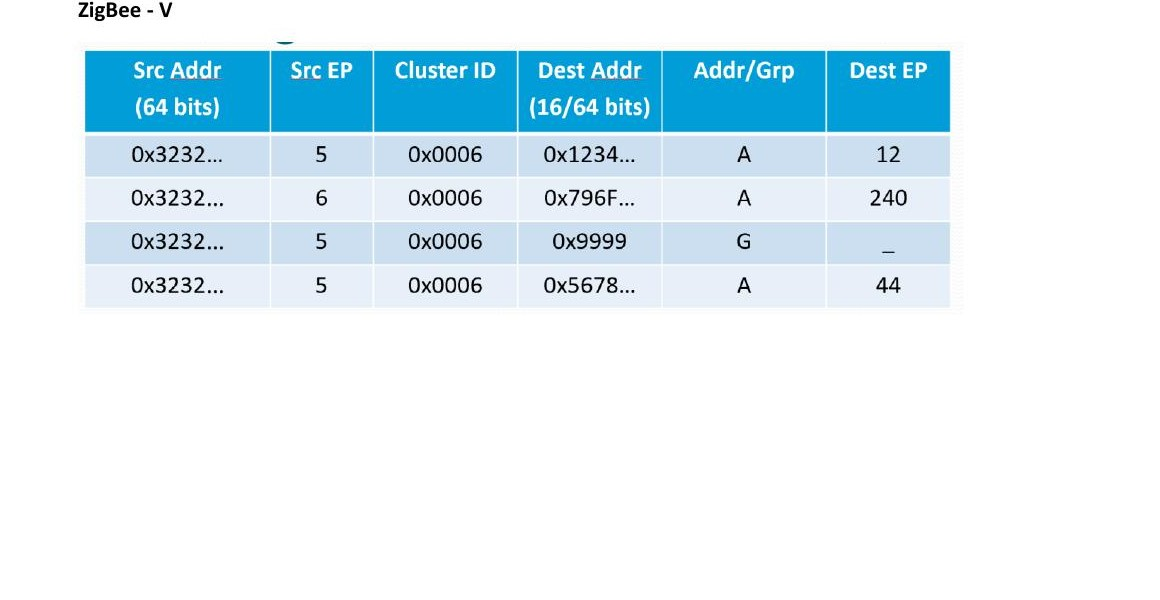
\includegraphics[keepaspectratio]{images/exam-chessa-zigbee-aps.jpg}}
\caption{Esempio di APS Binding Table: ogni entry mappa un endpoint
sorgente con cluster e destination address/endpoint.}
\end{figure}

L'\textbf{Application Support Sublayer (APS)} funge da livello di
trasporto leggero che eroga Data Service, Binding Service e Group
Management. L'APS filtra i pacchetti per scartare quelli destinati a
endpoint non registrati o profili non compatibili, e genera gli
acknowledgment end-to-end.

La tabella mostra la \textbf{APS Binding Table}, il meccanismo con cui
ZigBee implementa l'\textbf{indirizzamento indiretto}. Un dispositivo
sorgente (che conosce solo il proprio endpoint e il cluster di
interesse) non ha bisogno di conoscere l'indirizzo di rete del
destinatario: consulta la binding table.

Le colonne della tabella sono: - \textbf{Src Addr (64 bit)}: indirizzo
MAC a 64 bit del dispositivo sorgente. - \textbf{Src EP}: endpoint
sorgente (1--240). - \textbf{Cluster ID}: il cluster di riferimento (es.
\texttt{0x0006} = OnOff Cluster). - \textbf{Dest Addr (16/64 bit)}:
indirizzo di destinazione (short 16 bit o MAC 64 bit). -
\textbf{Addr/Grp}: \texttt{A} = indirizzo unicast, \texttt{G} =
indirizzo di gruppo (multicast). - \textbf{Dest EP}: endpoint
destinazione (vuoto per i gruppi).

Questo meccanismo è fondamentale: se un dispositivo cambia indirizzo di
rete a 16 bit (dopo un reset), l'APS usa la \textbf{Address Map Table}
(che associa indirizzi 16-bit agli immutabili MAC 64-bit) per
ripristinare i binding automaticamente. Il binding può essere
configurato solo su esplicita richiesta dello ZDO di un coordinatore o
di un router.

\begin{center}\rule{0.5\linewidth}{0.5pt}\end{center}

\section{Cluster e Binding tra Dispositivi (Modello
Client-Server)}\label{cluster-e-binding-tra-dispositivi-modello-client-server}

\begin{figure}
\centering
\pandocbounded{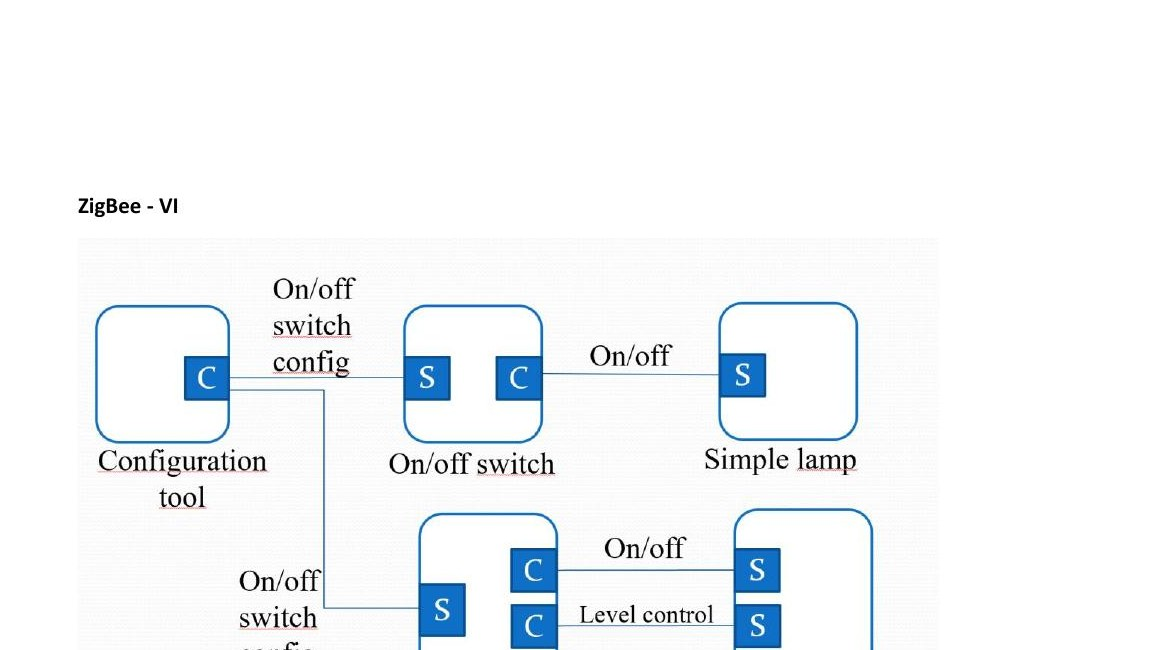
\includegraphics[keepaspectratio]{images/exam-chessa-zigbee-binding.jpg}}
\caption{Esempio di binding ZigBee: Configuration tool configura un
on/off switch, che controlla una Simple lamp e un Dimmer switch, il
quale controlla una Dimmable lamp.}
\end{figure}

La \textbf{ZigBee Cluster Library (ZCL)} introduce un modello gerarchico
Client-Server per l'accesso e la manipolazione di un Dominio Funzionale.
Lo schema illustra come il binding colleghi dispositivi tramite cluster.
Ogni rettangolo contiene le lettere C (Client) o S (Server) per ciascun
cluster supportato.

\begin{itemize}
\tightlist
\item
  \textbf{Il Server} è colui che ospita fisicamente lo stato (memorizza
  gli \textbf{attributi}).
\item
  \textbf{Il Client} è il dispositivo che invia comandi per manipolare
  gli attributi sul Server.
\end{itemize}

Nell'esempio: - La \textbf{Configuration tool} (solo C) si lega
all'\textbf{On/off switch} (S+C) per configurarlo. - L'\textbf{On/off
switch} (come client) controlla la \textbf{Simple lamp} (S = solo server
OnOff). - Il \textbf{Dimmer switch} (S+C) riceve configurazioni (S) e
controlla la \textbf{Dimmable lamp} che implementa sia OnOff (S) che
Level Control (S).

Il binding è unidirezionale: si va da client a server. Viene creato
tramite \texttt{BIND.request} allo ZDO e memorizzato nella binding table
dell'APS. Un singolo client può essere legato a più server (fan-out).

\begin{center}\rule{0.5\linewidth}{0.5pt}\end{center}

\section{Lo ZigBee Device Object
(ZDO)}\label{lo-zigbee-device-object-zdo}

Lo \textbf{ZDO} è la speciale applicazione gestionale del nodo attaccata
all'Endpoint 0. I principali servizi esposti includono: - \textbf{Device
e Service Discovery}: recupera indirizzi fisici/rete e informazioni sui
servizi. - \textbf{Binding Management}: processa e attua fisicamente
tutte le richieste di modifica alle tabelle di binding dell'APS. -
\textbf{Node e Network Management}: gestisce join, leave e lo
smistamento di informazioni sulle routing table.

\newpage

\chapter{IoT Design (Appunti d'Esame)}\label{iot-design-appunti-desame}

\section{Duty Cycle e Efficienza
Energetica}\label{duty-cycle-e-efficienza-energetica}

La soluzione alla sfida energetica nell'IoT si chiama \textbf{duty
cycle} (ciclo di lavoro). Il duty cycle è la frazione di un periodo in
cui il sistema (o un suo componente) è attivo. L'idea è di sfruttare i
periodi di inattività per mettere in sleep tutti i componenti possibili,
riducendo al minimo il consumo. Applicarlo in modo aggressivo è la leva
principale per estendere la vita della batteria, attivando ogni
componente \textbf{solo quando strettamente necessario}.

\subsection{Esempio pratico: il codice Arduino e Calcolo del Duty
Cycle}\label{esempio-pratico-il-codice-arduino-e-calcolo-del-duty-cycle}

\begin{figure}
\centering
\pandocbounded{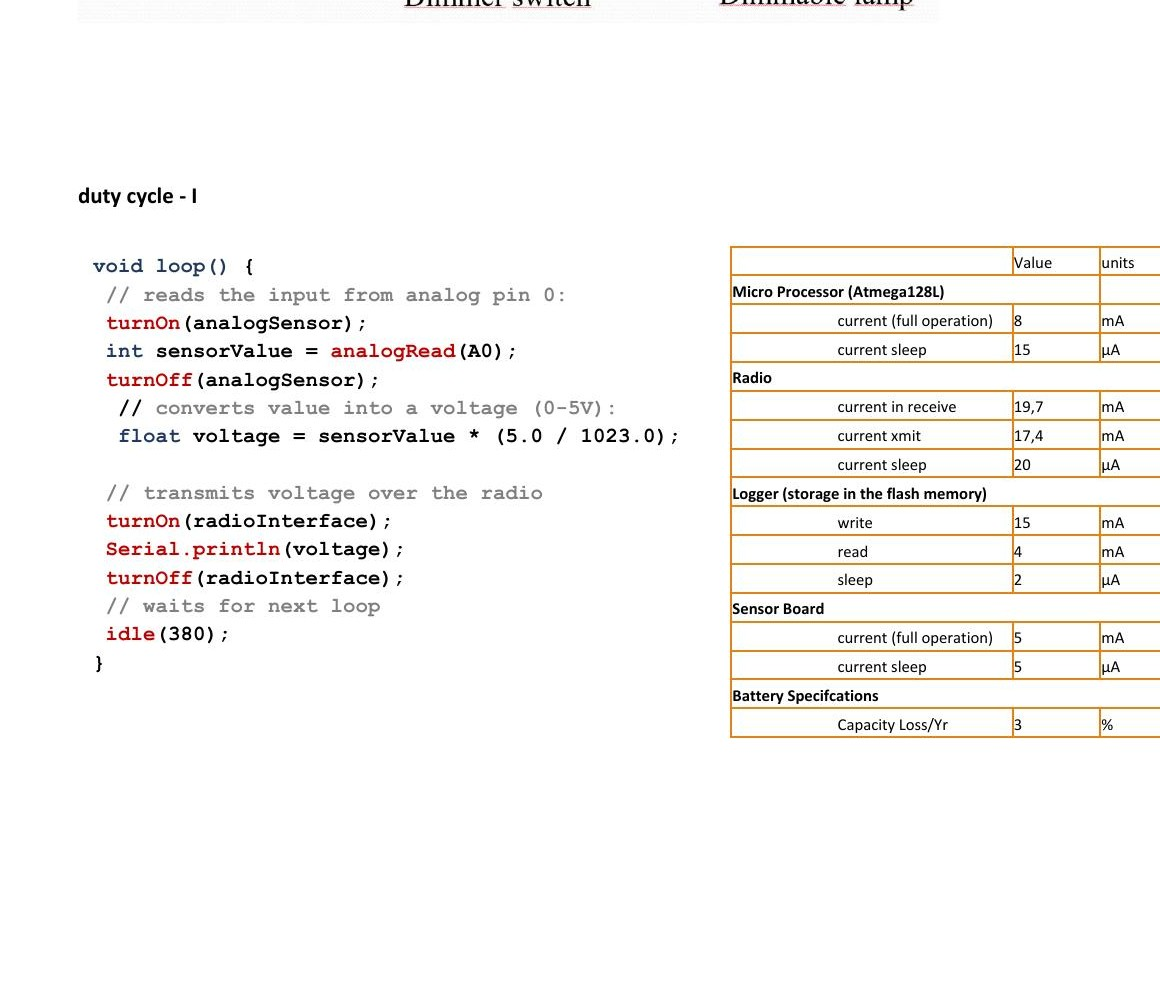
\includegraphics[keepaspectratio]{images/exam-chessa-dutycycle-code.jpg}}
\caption{Codice Arduino che implementa il duty cycling selettivo dei
componenti (sensore, radio) e tabella dei consumi in mA per componente e
stato.}
\end{figure}

Il codice mostra il pattern classico per minimizzare i consumi spegnendo
esplicitamente ogni componente quando non serve:

\begin{Shaded}
\begin{Highlighting}[]
\DataTypeTok{void}\NormalTok{ loop}\OperatorTok{()} \OperatorTok{\{}
\NormalTok{    turnOn}\OperatorTok{(}\NormalTok{analogSensor}\OperatorTok{);}   \CommentTok{// sensore acceso solo durante lettura}
    \DataTypeTok{int}\NormalTok{ sensorValue }\OperatorTok{=}\NormalTok{ analogRead}\OperatorTok{(}\NormalTok{A0}\OperatorTok{);} \CommentTok{// lettura}
\NormalTok{    turnOff}\OperatorTok{(}\NormalTok{analogSensor}\OperatorTok{);}  \CommentTok{// sensore spento}
    
    \DataTypeTok{float}\NormalTok{ voltage }\OperatorTok{=}\NormalTok{ sensorValue }\OperatorTok{*} \OperatorTok{(}\FloatTok{5.0} \OperatorTok{/} \FloatTok{1023.0}\OperatorTok{);}
    
\NormalTok{    turnOn}\OperatorTok{(}\NormalTok{radioInterface}\OperatorTok{);} \CommentTok{// radio accesa solo durante trasmissione}
\NormalTok{    Serial}\OperatorTok{.}\NormalTok{println}\OperatorTok{(}\NormalTok{voltage}\OperatorTok{);}
\NormalTok{    turnOff}\OperatorTok{(}\NormalTok{radioInterface}\OperatorTok{);}
    
\NormalTok{    idle}\OperatorTok{(}\DecValTok{380}\OperatorTok{);}  \CommentTok{// MCU in sleep per 380 ms}
\OperatorTok{\}}
\end{Highlighting}
\end{Shaded}

Usando i valori della tabella (es. Tmote Sky): - \textbf{Processore}:
attivo 8 mA, sleep 15 μA - \textbf{Radio}: TX 17.4 mA, RX 19.7 mA, sleep
20 μA - \textbf{Sensore}: attivo 5 mA, sleep 5 μA

Il duty cycle di ciascun componente si calcola come:
\[DC_\text{componente} = \frac{t_\text{attivo}}{T_\text{periodo}}\]

Se le operazioni di sensing + TX durano \textasciitilde20 ms e il ciclo
totale è 400 ms, il duty cycle della radio è \(20/400 = 5\%\). La
corrente media risultante è molto inferiore alla corrente di picco,
estendendo la vita della batteria di ordini di grandezza. La perdita di
capacità della batteria del 3\%/anno indica che anche con battery
standby c'è un degrado nel tempo.

\begin{center}\rule{0.5\linewidth}{0.5pt}\end{center}

\section{Effetto del duty cycle sulla vita della
batteria}\label{effetto-del-duty-cycle-sulla-vita-della-batteria}

\begin{figure}
\centering
\pandocbounded{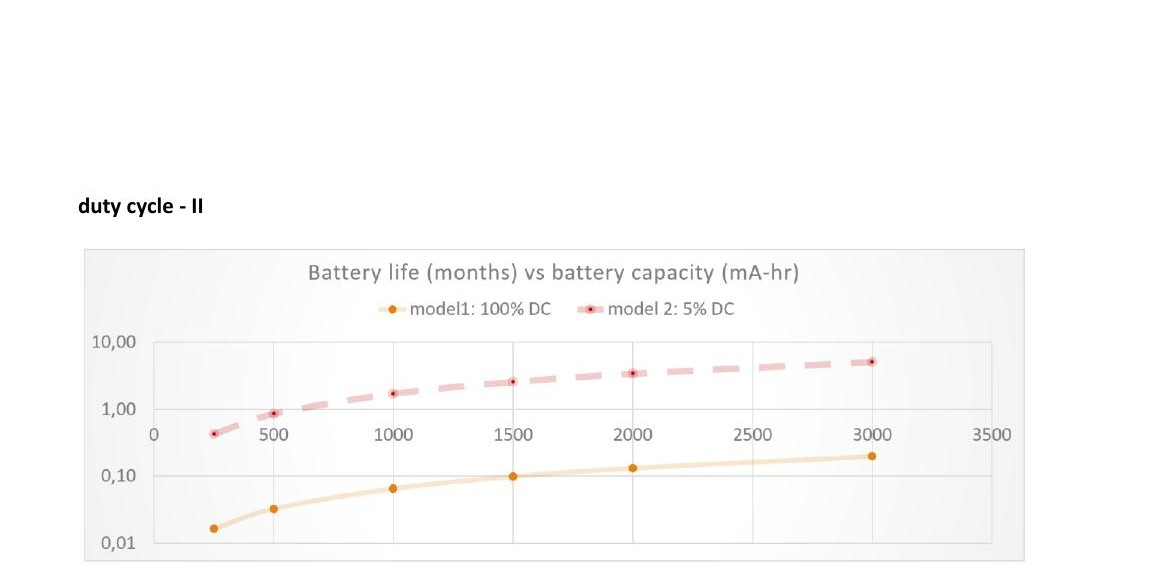
\includegraphics[keepaspectratio]{images/exam-chessa-dutycycle-graph.jpg}}
\caption{Grafico log-log: vita della batteria (mesi) vs capacità della
batteria (mAh) per duty cycle 100\% (model1) e 5\% (model2).}
\end{figure}

Il grafico mostra l'impatto del duty cycle sulla vita della batteria in
scala logaritmica. Due modelli a confronto:

\begin{itemize}
\tightlist
\item
  \textbf{Model 1 (100\% DC)}: il dispositivo è sempre attivo. La vita
  della batteria scala linearmente con la capacità ma rimane nell'ordine
  dei mesi (0.01--0.3 mesi per capacità 500--3000 mAh).
\item
  \textbf{Model 2 (5\% DC)}: il dispositivo è attivo solo il 5\% del
  tempo. La vita si estende di un fattore \textasciitilde20: con la
  stessa batteria, si passa da 0.1 a circa 2--8 mesi.
\end{itemize}

La scala logaritmica rivela che la relazione vita-capacità non è
lineare: il duty cycle agisce moltiplicativamente. Ridurre il duty cycle
da 100\% a 5\% equivale a moltiplicare la capacità effettiva della
batteria per 20.

\textbf{Conclusione progettuale}: per applicazioni IoT con autonomia di
anni, ridurre il duty cycle è molto più efficace che aumentare la
capacità della batteria. Una batteria da 3000 mAh a 5\% DC dura circa 8
mesi; per durare anni si deve abbassare ulteriormente il duty cycle o
usare energy harvesting. Ad alti DC, aumentare la capacità della
batteria ha un effetto quasi trascurabile.

\newpage

\chapter{MAC Protocols (Appunti
d'Esame)}\label{mac-protocols-appunti-desame}

Nei sistemi IoT, il protocollo MAC deve minimizzare il consumo
energetico riducendo il \textbf{duty cycle}. Esistono vari approcci, tra
cui la sincronizzazione (S-MAC) e il preamble sampling (B-MAC, X-MAC).

\section{Sincronizzazione: S-MAC
(Sensor-MAC)}\label{sincronizzazione-s-mac-sensor-mac}

\begin{figure}
\centering
\pandocbounded{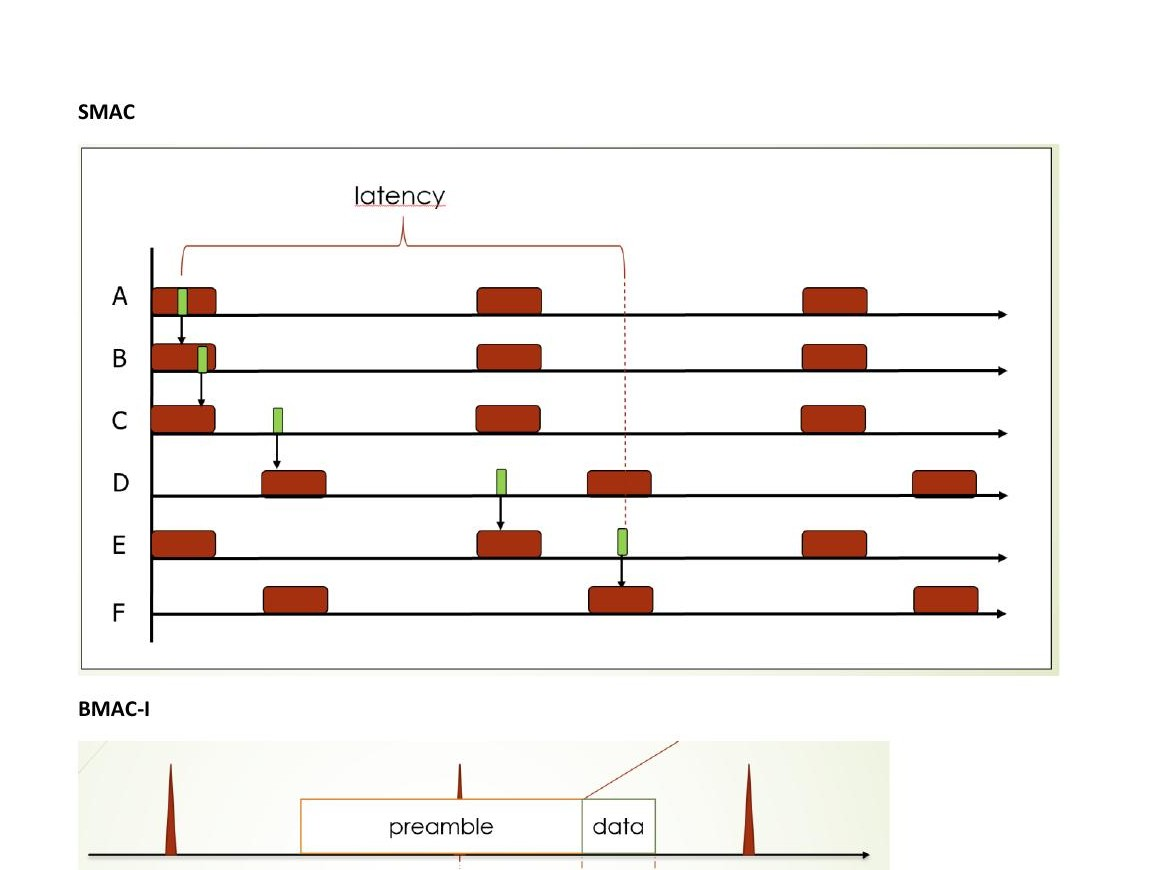
\includegraphics[keepaspectratio]{images/exam-chessa-smac.jpg}}
\caption{S-MAC: i nodi A--F hanno schedule sincronizzati (verde =
listen, rosso = active/TX). La latenza multi-hop si accumula: il
pacchetto da A deve aspettare i periodi di ascolto di ogni hop
successivo.}
\end{figure}

\textbf{S-MAC} riduce il consumo energetico tramite
\textbf{sincronizzazione locale}: nodi vicini si accordano su un periodo
di ascolto comune (listen period) e dormono nel resto del tempo.

\textbf{Meccanismo}: 1. Ogni nodo trasmette periodicamente un pacchetto
\textbf{SYNC} che annuncia il proprio schedule. 2. I vicini che ricevono
il SYNC adottano lo stesso schedule o mantengono il proprio e
memorizzano quello del vicino. 3. Nel \textbf{listen period}: esecuzione
di CSMA/CA con RTS/CTS prima di trasmettere. 4. Nel \textbf{sleep
period}: la radio è spenta.

\textbf{Problema della latenza multi-hop}: in un percorso multi-hop,
ogni nodo deve aspettare il periodo di ascolto del nodo successivo. La
latenza totale si accumula ad ogni salto (es. latenza proporzionale a
\(n \cdot t_{sleep}/2\)). \textbf{Adaptive duty cycle}: per mitigare
questo, se un nodo riceve un RTS o CTS in sorveglianza, capisce che c'è
traffico nelle vicinanze e mantiene la radio accesa per il resto della
trasmissione, anticipando che potrebbe essere il prossimo hop.

\begin{center}\rule{0.5\linewidth}{0.5pt}\end{center}

\section{Preamble Sampling: B-MAC}\label{preamble-sampling-b-mac}

\begin{figure}
\centering
\pandocbounded{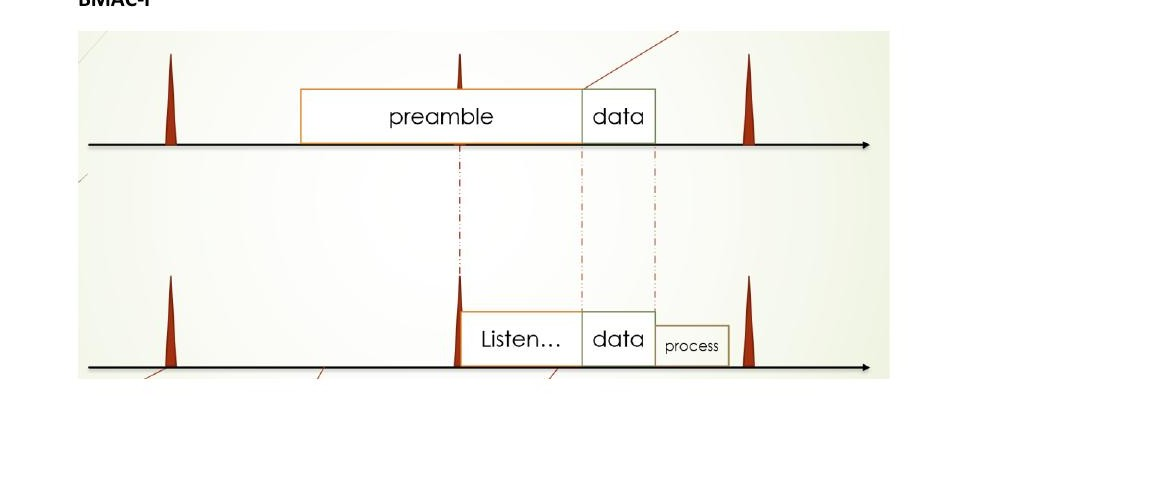
\includegraphics[keepaspectratio]{images/exam-chessa-bmac.jpg}}
\caption{B-MAC: il mittente (in alto) invia un lungo preamble seguito
dai data; il ricevitore (in basso) si sveglia, ascolta, individua il
preamble, rimane sveglio e riceve i data.}
\end{figure}

\textbf{B-MAC} usa il \textbf{preamble sampling} (Low Power Listening,
LPL) ed elimina del tutto la sincronizzazione:

\begin{itemize}
\tightlist
\item
  \textbf{Lato ricevitore}: si sveglia periodicamente (ogni
  \(t_{check}\)), campiona il canale per un breve istante. Se rileva il
  preambolo, rimane sveglio e riceve i dati; altrimenti si riaddormenta
  subito.
\item
  \textbf{Lato mittente}: quando deve trasmettere, invia un
  \textbf{preambolo lungo} per una durata \(> t_{check}\), per garantire
  che qualunque sia il momento in cui il ricevitore si sveglia, trovi il
  preambolo ``in aria''. Dopo il preambolo, invia i dati effettivi.
\end{itemize}

\textbf{Trade-off e Ottimizzazione}:
\pandocbounded{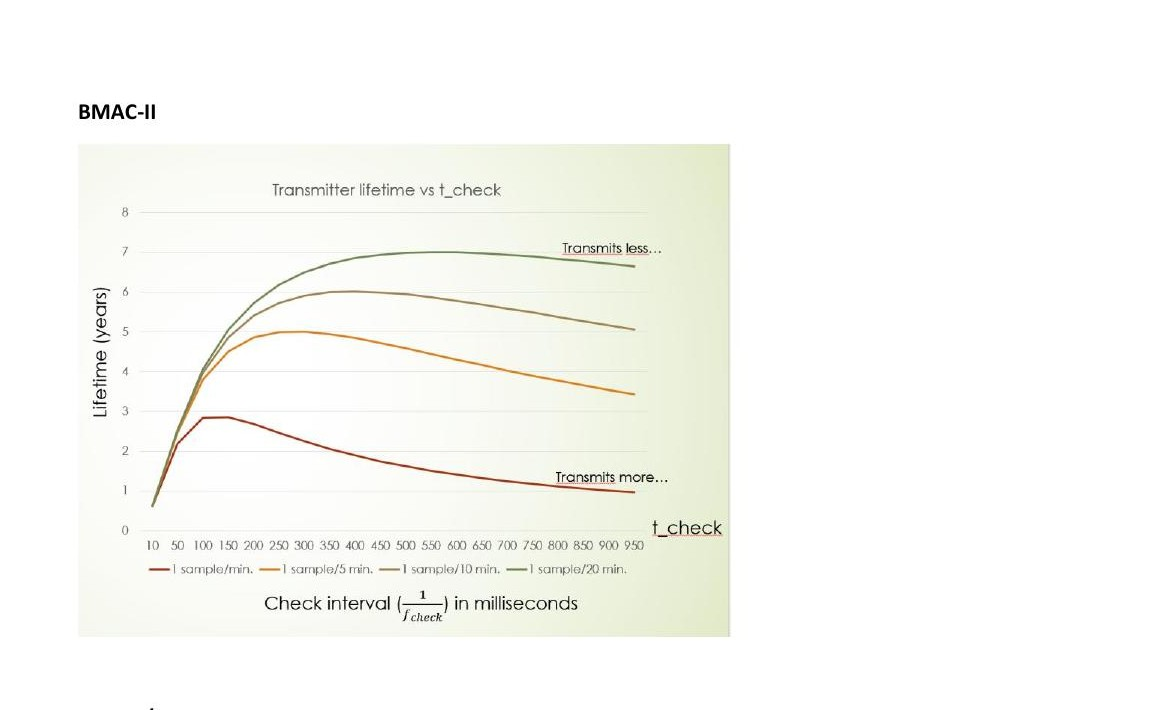
\includegraphics[keepaspectratio]{images/exam-chessa-bmac-graph.jpg}}
\emph{Fig. --- Grafico B-MAC: vita del trasmettitore (anni) vs
intervallo di check t\_check (ms), per diverse frequenze di
campionamento (1 sample/min, 1/5 min, 1/10 min, 1/20 min).}

Il trade-off fondamentale riguarda come la frequenza di trasmissione e
\(t_{check}\) influenzano la batteria del \textbf{trasmettitore}. Al
crescere di \(t_{check}\), il preambolo deve essere più lungo, quindi il
trasmettitore consuma di più per ogni trasmissione. Tuttavia, la vita
del trasmettitore ha un \textbf{massimo} per un valore ottimale di
\(t_{check}\): - \(t_{check}\) troppo breve → il ricevitore si sveglia
spesso, preambolo corto (basso overhead per TX ma alto per RX). -
\(t_{check}\) troppo lungo → preambolo lunghissimo, overhead troppo alto
per il TX.

\begin{center}\rule{0.5\linewidth}{0.5pt}\end{center}

\section{Evoluzione: X-MAC vs B-MAC}\label{evoluzione-x-mac-vs-b-mac}

\begin{figure}
\centering
\pandocbounded{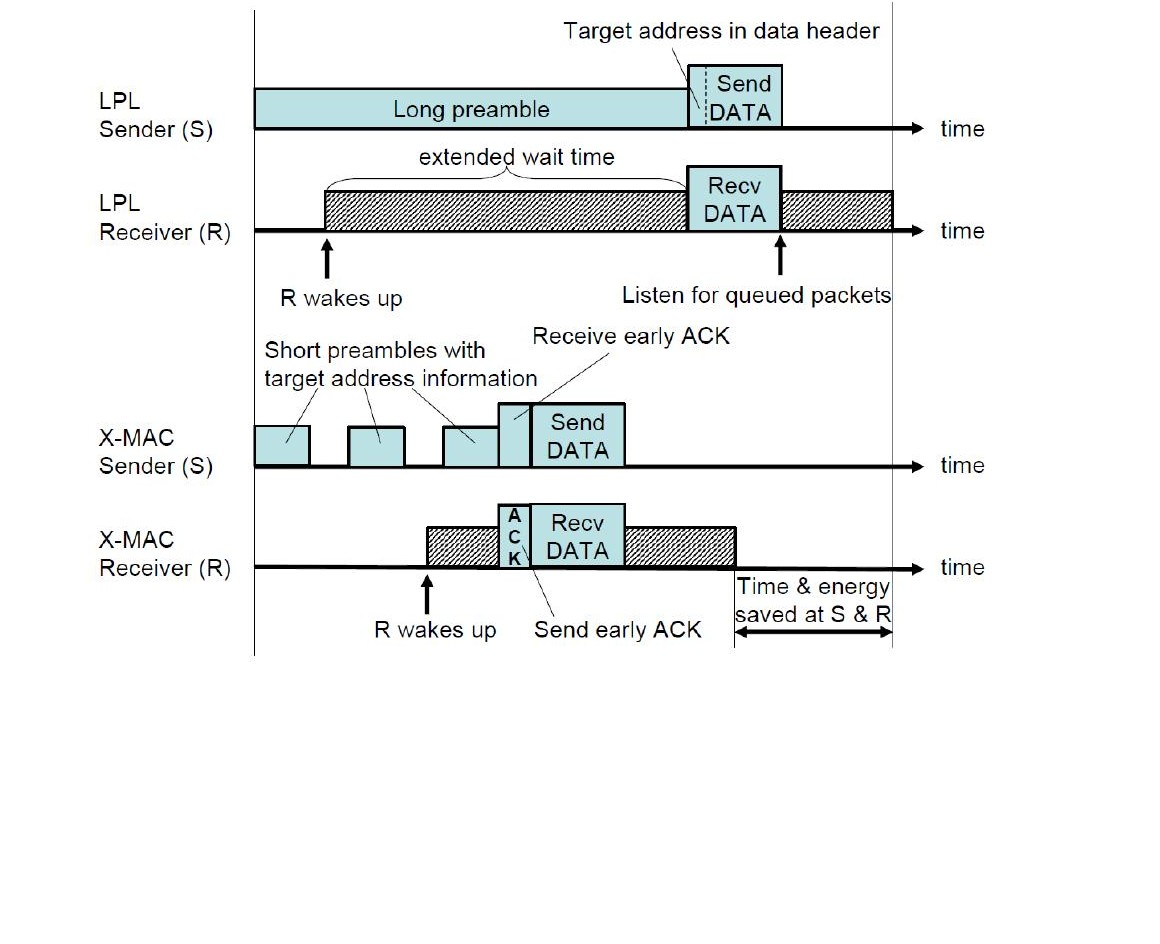
\includegraphics[keepaspectratio]{images/exam-chessa-xmac.jpg}}
\caption{Confronto LPL (B-MAC, righe superiori) e X-MAC (righe
inferiori): X-MAC usa preamble corti con indirizzo target; il ricevitore
invia early ACK; mittente e ricevitore risparmiano tempo ed energia.}
\end{figure}

\textbf{X-MAC} migliora B-MAC risolvendo lo spreco energetico del
preambolo lungo e l'overhearing (nodi non destinatari che restano svegli
inutilmente durante il lungo preambolo):

\begin{itemize}
\tightlist
\item
  \textbf{Mittente}: invia una sequenza di \textbf{short preambles}
  (strobe) contenenti ciascuno l'indirizzo del destinatario target.
\item
  \textbf{Ricevitore target}: si sveglia, legge il proprio indirizzo nel
  preambolo, e invia immediatamente un \textbf{early ACK}.
\item
  \textbf{Mittente}: ricevendo l'ACK, interrompe i preamboli e trasmette
  subito i dati.
\item
  I \textbf{non-destinatari} vedono il proprio indirizzo assente nel
  preambolo e si riaddormentano subito.
\end{itemize}

Il risultato è un forte risparmio sia per il mittente (preambolo più
corto in media) sia per il ricevitore (meno overhearing).

\newpage

\chapter{Lo Standard IEEE 802.15.4}\label{lo-standard-ieee-802.15.4}

Lo standard IEEE 802.15.4 definisce le specifiche del \textbf{physical
layer} e del \textbf{MAC layer} per le \textbf{Low-Rate Wireless
Personal Area Network} (\emph{LR-WPAN}, reti personali senza fili a
bassa velocità). L'obiettivo è fornire un protocollo radio
standardizzato per dispositivi a risorse limitate --- sensori,
attuatori, nodi IoT --- che richiedono bassi consumi energetici
piuttosto che elevate velocità di trasmissione.

\section{IEEE 802.15.4 - I (Struttura del
Superframe)}\label{ieee-802.15.4---i-struttura-del-superframe}

\begin{figure}
\centering
\pandocbounded{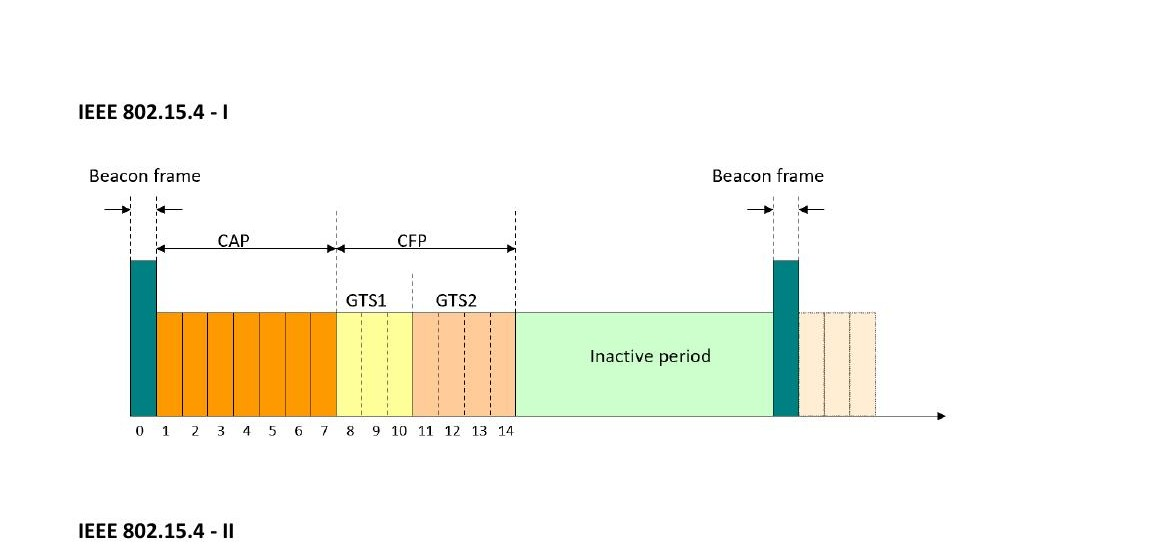
\includegraphics[keepaspectratio]{images/exam-chessa-ieee802154-superframe.jpg}}
\caption{Struttura del superframe IEEE 802.15.4: Beacon frame → CAP
(Contention Access Period, slot 0--6) → CFP (Contention Free Period,
GTS1 e GTS2, slot 7--11) → Inactive period (slot 12--14) → prossimo
Beacon.}
\end{figure}

La modalità \emph{beacon-enabled} struttura il tempo in
\textbf{superframe}, delimitati dall'invio periodico di un frame beacon
da parte del PAN coordinator. Il superframe divide il tempo in due
porzioni: una \textbf{active period} e una \textbf{inactive period}.
Durante il periodo inattivo il PAN coordinator e i dispositivi connessi
possono entrare in modalità a basso consumo (sleep).

La \textbf{active period} comprende fino a \textbf{16 time slot} di
uguale dimensione, suddivisi in:

\begin{itemize}
\tightlist
\item
  \textbf{Beacon frame}: il coordinatore trasmette periodicamente un
  beacon che annuncia l'inizio del superframe, contiene i parametri
  della rete e la lista dei dispositivi con dati pendenti.
\item
  \textbf{CAP} (\emph{Contention Access Period}): fino a 15 slot. I
  dispositivi competono per il canale usando il protocollo
  \textbf{CSMA-CA a slot} (\emph{slotted CSMA-CA}). Un dispositivo
  attende un numero casuale di slot; se il canale è occupato riprova
  dopo un altro backoff casuale; se è libero trasmette e mantiene il
  canale fino alla fine del frame. Usato per traffico non deterministico
  (dati aperiodici).
\item
  \textbf{CFP} (\emph{Contention Free Period}): opzionale, occupa gli
  ultimi slot del periodo attivo. Diviso in \textbf{GTS}
  (\emph{Guaranteed Time Slot}), ciascuno assegnato dal PAN coordinator
  a una specifica applicazione per comunicazioni deterministiche a bassa
  latenza. Il GTS è accessibile senza CSMA-CA, garantendo latenza
  deterministica. Ogni CFP può contenere al massimo 7 GTS, ciascuno
  composto da uno o più slot.
\end{itemize}

\textbf{Inactive period}: tutti i dispositivi (incluso il coordinatore)
possono dormire per risparmiare energia. La durata del periodo inattivo
determina il duty cycle della rete: un inactive period lungo → basso
duty cycle → lunga vita della batteria → latenza più alta.

\begin{calloutwarning}{Il CAP non può essere eliminato}

Anche quando è presente il CFP, il CAP è necessario per il mantenimento
della rete: gestione di associazioni/disassociazioni, richieste di GTS,
ecc. Tutte le transazioni basate su contesa devono completarsi prima
dell'inizio del CFP. Un dispositivo che trasmette in un GTS deve
completare la trasmissione entro il suo GTS assegnato.

\end{calloutwarning}

\begin{center}\rule{0.5\linewidth}{0.5pt}\end{center}

\section{IEEE 802.15.4 - II (Indirect Data
Transfer)}\label{ieee-802.15.4---ii-indirect-data-transfer}

\begin{figure}
\centering
\pandocbounded{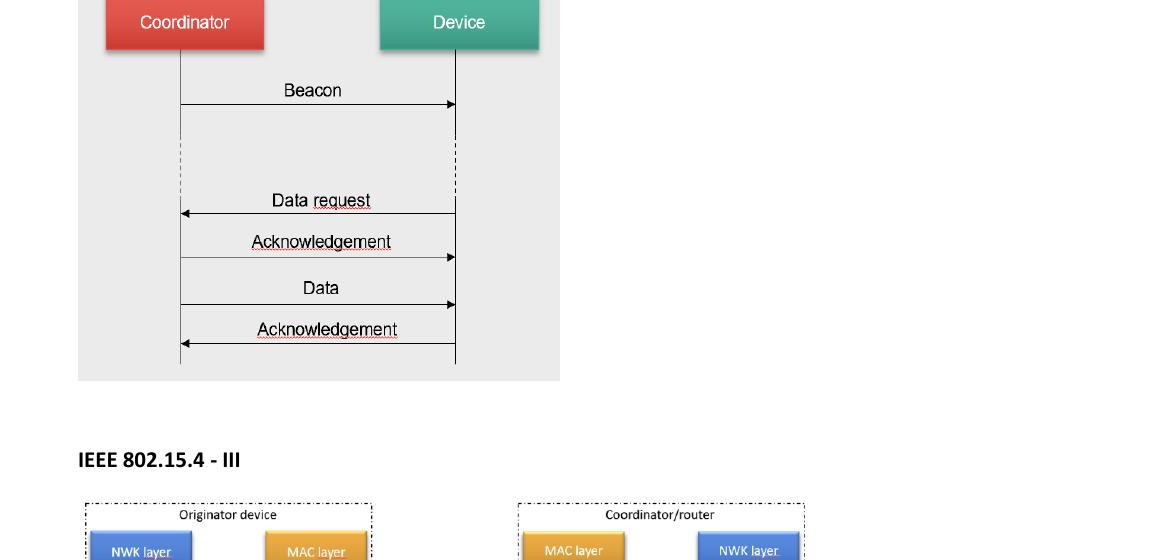
\includegraphics[keepaspectratio]{images/exam-chessa-ieee802154-indirect.jpg}}
\caption{Trasferimento dati indiretto in IEEE 802.15.4: il dispositivo
si sveglia al beacon, invia una Data request al coordinatore, riceve ACK
e poi i dati.}
\end{figure}

Il trasferimento \textbf{indiretto} è usato quando il destinatario è un
dispositivo che dorme la maggior parte del tempo (RFD, end-device). Il
coordinatore non può trasmettere dati in modo asincrono perché il
dispositivo potrebbe essere in sleep.

\textbf{Da coordinatore a end-device}: 1. Il \textbf{coordinatore}
memorizza il messaggio e trasmette un \textbf{Beacon} che include (nella
lista \emph{pending addresses}) l'indirizzo dei dispositivi per cui ha
dati in coda. 2. Il \textbf{dispositivo}, che dorme la maggior parte del
tempo, si sveglia al beacon, ascolta occasionalmente il beacon, legge la
lista, se vede il proprio indirizzo invia una \textbf{Data request} al
coordinatore nel CAP. 3. Il \textbf{coordinatore} risponde con un
\textbf{Acknowledgement} immediato. 4. Il \textbf{coordinatore}
trasmette i \textbf{dati} accodati in uno slot successivo del CAP. 5. Il
\textbf{dispositivo} risponde con un \textbf{Acknowledgement}
obbligatorio. 6. Infine il coordinatore rimuove il messaggio dalla
lista.

Il device può poi tornare in sleep. Il vantaggio è che il dispositivo
non deve rimanere sveglio ad aspettare dati: si sveglia solo al beacon
(duty cycle controllato), controlla se ci sono dati per lui, li recupera
e dorme di nuovo.

\begin{center}\rule{0.5\linewidth}{0.5pt}\end{center}

\section{IEEE 802.15.4 - III (Protocollo di
Associazione)}\label{ieee-802.15.4---iii-protocollo-di-associazione}

\begin{figure}
\centering
\pandocbounded{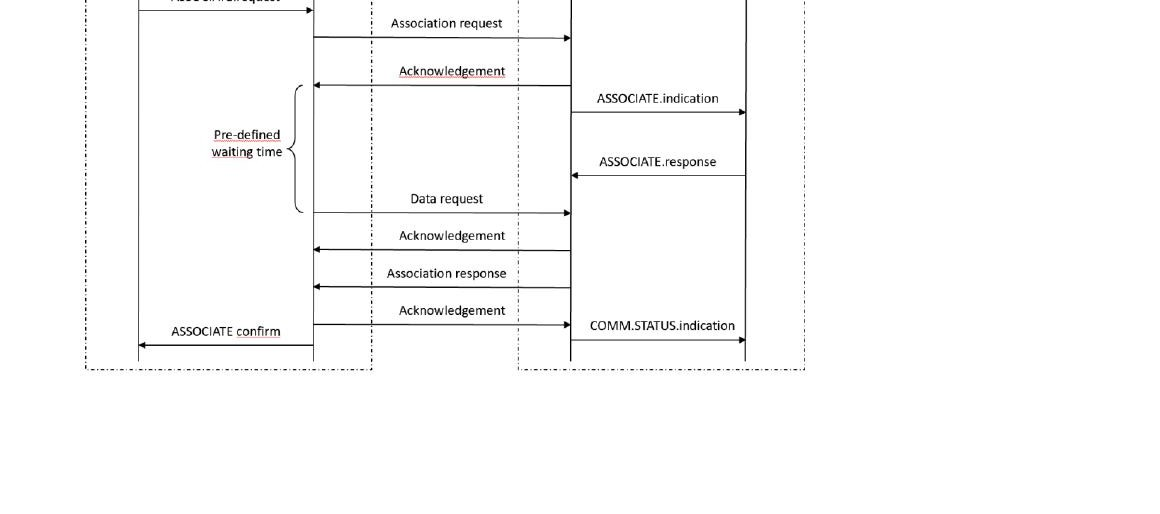
\includegraphics[keepaspectratio]{images/exam-chessa-ieee802154-association.jpg}}
\caption{Protocollo di associazione IEEE 802.15.4: sequenza di messaggi
tra NWK e MAC layer del dispositivo (sinistra) e del coordinatore/router
(destra).}
\end{figure}

L'associazione è il processo con cui un dispositivo entra a far parte di
una PAN. È pensata per reti beacon-enabled e si compone di una fase sul
lato end-device e una sul lato coordinatore. Lo schema mostra il
protocollo di \textbf{associazione} visto a livello di primitives
NWK-MAC.

\subsection{Lato End-Device}\label{lato-end-device}

Il dispositivo che vuole associarsi deve aver identificato in anticipo
la PAN di destinazione attraverso il servizio \textbf{SCAN} (scansione
attiva).

\begin{enumerate}
\def\labelenumi{\arabic{enumi}.}
\tightlist
\item
  Il NWK del dispositivo emette \texttt{ASSOCIATE.request} al proprio
  MAC layer. Prende come parametri l'identificatore di PAN, l'indirizzo
  del coordinatore e il proprio indirizzo IEEE a 64 bit esteso.
\item
  Il MAC invia un \textbf{Association request} frame al coordinatore. La
  richiesta viene inviata nel CAP usando CSMA-CA a slot.
\item
  Il coordinatore MAC risponde con \textbf{Acknowledgement} immediato
  --- ma questo non implica che la richiesta sia stata accettata.
\end{enumerate}

\subsection{Lato Coordinatore e
Completamento}\label{lato-coordinatore-e-completamento}

Dopo aver ricevuto la richiesta, il MAC layer del coordinatore emette
\textbf{ASSOCIATE.indication} verso il network layer (NWK), che decide
se accettare o rifiutare. In caso di accettazione, il NWK layer:

\begin{enumerate}
\def\labelenumi{\arabic{enumi}.}
\setcounter{enumi}{3}
\tightlist
\item
  Il coordinatore NWK riceve \texttt{ASSOCIATE.indication} e prepara la
  risposta con \texttt{ASSOCIATE.response}, selezionando un
  \textbf{indirizzo a 16 bit} che il dispositivo utilizzerà in futuro al
  posto dell'indirizzo a 64 bit.
\item
  Il dispositivo aspetta un \textbf{pre-defined waiting time} (il
  coordinatore deve elaborare la richiesta e decidere se accettarla). Il
  MAC layer invia la risposta di associazione usando
  \textbf{trasmissione indiretta}.
\item
  Il dispositivo MAC invia una \textbf{Data request} per recuperare la
  risposta del coordinatore.
\item
  Il coordinatore MAC risponde con \textbf{Acknowledgement} +
  \textbf{Association response} (contenente l'indirizzo a 16 bit
  assegnato e lo status della richiesta).
\item
  Il dispositivo MAC invia \textbf{Acknowledgement} finale.
\item
  Il dispositivo NWK riceve \texttt{ASSOCIATE\ confirm} con l'indirizzo
  assegnato.
\item
  Il coordinatore NWK riceve \texttt{COMM.STATUS.indication}, segnalando
  che l'associazione è conclusa --- con successo o con un codice di
  errore.
\end{enumerate}

\newpage

\chapter{Embedded Programming e
Arduino}\label{embedded-programming-e-arduino}

\section{Modelli di Programmazione per
Embedded}\label{modelli-di-programmazione-per-embedded}

Il problema della gestione dell'I/O con memoria limitata ha portato allo
sviluppo di diversi modelli di programmazione. I due esempi principali
sono il \textbf{modello Arduino} (event loop sincrono) e il
\textbf{modello TinyOS} (eventi + task asincroni).

\subsection{Il Modello Arduino}\label{il-modello-arduino}

\begin{figure}
\centering
\pandocbounded{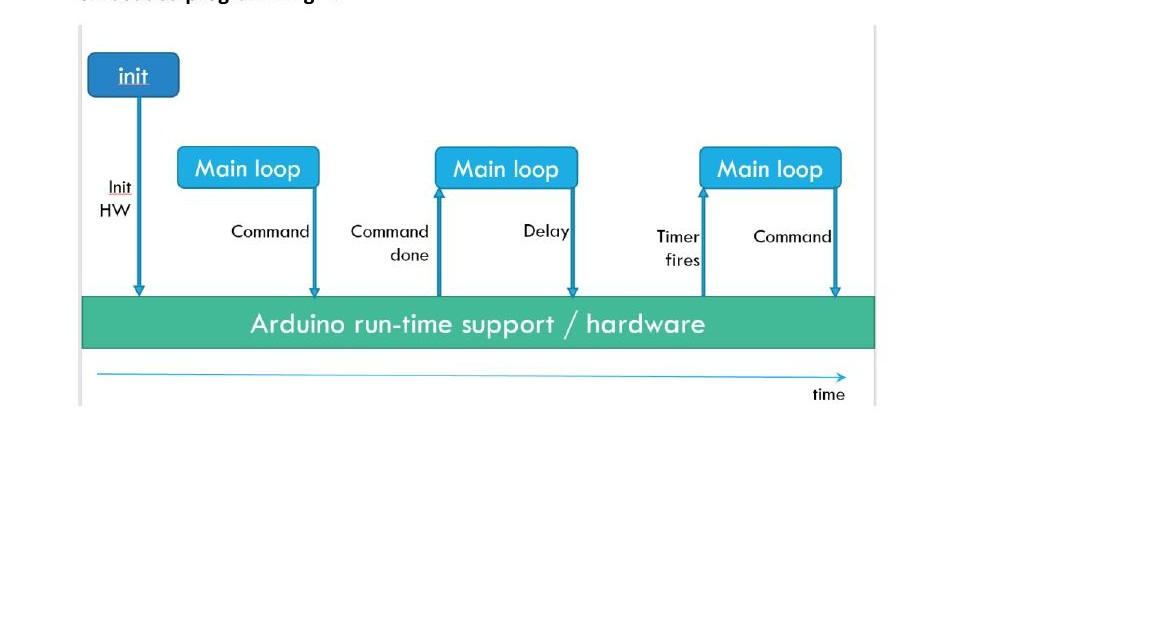
\includegraphics[keepaspectratio]{images/exam-chessa-embedded-arduino.jpg}}
\caption{Modello di esecuzione Arduino: init → loop() ripetuto. I
comandi attivano l'hardware; delay() aspetta; il timer fires avvia la
ripetizione.}
\end{figure}

Arduino adotta un approccio estremamente semplice: il lavoro è definito
in una singola funzione \texttt{loop()}, eseguita ripetutamente da
\textbf{un unico thread}. Non c'è sospensione del thread, non ci sono
context switch.

\begin{enumerate}
\def\labelenumi{\arabic{enumi}.}
\tightlist
\item
  \textbf{init}: la funzione \texttt{setup()} viene eseguita una sola
  volta all'avvio. Inizializza l'hardware, configura i pin, prepara le
  comunicazioni seriali.
\item
  \textbf{Main loop}: la funzione \texttt{loop()} viene invocata
  ripetutamente all'infinito dal runtime Arduino.
\item
  \textbf{Command}: dentro \texttt{loop()}, il codice interagisce con
  l'hardware tramite comandi sincroni (es. \texttt{analogRead()},
  \texttt{Serial.println()}).
\item
  \textbf{Delay}: \texttt{delay(ms)} blocca l'esecuzione per il tempo
  specificato (busy waiting o sleep), poi il timer fires riavvia il
  loop.
\end{enumerate}

Il modello è semplice ma \textbf{bloccante}: durante \texttt{delay()} il
processore non può fare altro. Se un'operazione di I/O richiede tempo,
si aspetta semplicemente che si completi. Gli interrupt possono
intervenire anche durante il delay, ma il thread principale rimane
sospeso.

\subsection{Il Modello TinyOS}\label{il-modello-tinyos}

\begin{figure}
\centering
\pandocbounded{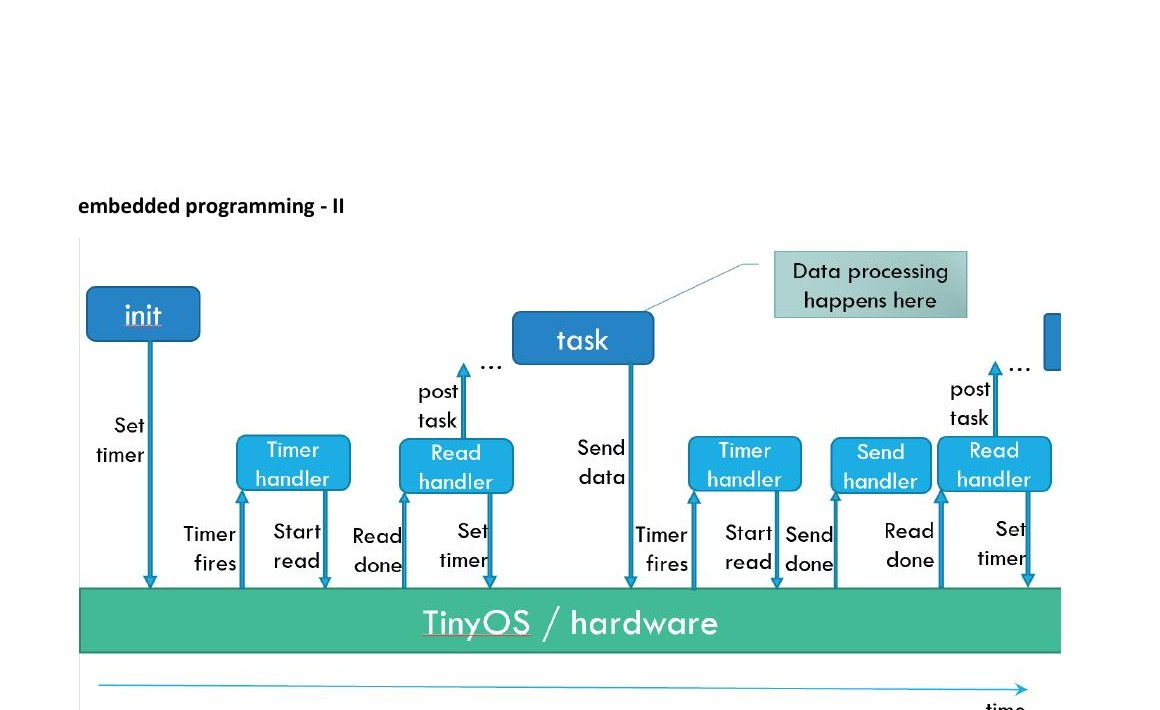
\includegraphics[keepaspectratio]{images/exam-chessa-embedded-tinyos.jpg}}
\caption{Modello di esecuzione TinyOS: catena di eventi (Timer → Read →
task → Send) senza loop bloccante. Il data processing avviene nel task
asincrono.}
\end{figure}

TinyOS usa un modello \textbf{event-driven} con componenti e interfacce,
progettato per massimizzare l'efficienza energetica e gestire attività
indipendenti senza sprecare memoria per i contesti dei thread. Non
esiste un loop bloccante: il sistema è guidato dagli eventi hardware. La
catena tipica:

\begin{enumerate}
\def\labelenumi{\arabic{enumi}.}
\tightlist
\item
  \textbf{init}: configura timer e hardware.
\item
  \textbf{Timer handler} (evento): scatta quando il timer fires → avvia
  una lettura dal sensore (\texttt{Start\ read}).
\item
  \textbf{Read handler} (evento): scatta quando la lettura è completata
  (\texttt{Read\ done}) → posta un task per il processing.
\item
  \textbf{task}: elabora i dati (\emph{Data processing happens here}) →
  avvia la trasmissione radio. I task sono unità di elaborazione
  non-preemptive eseguite sequenzialmente. Un task non aspetta mai
  (salva memoria).
\item
  \textbf{Send handler} (evento): scatta quando la trasmissione è
  completa → riconfigura il timer per il prossimo ciclo.
\end{enumerate}

\textbf{Vantaggi del modello event-driven}: - Nessun busy waiting: il
processore dorme tra un evento e l'altro. - Nessuno stack multiplo: un
unico stack (run-to-completion semantics). - Efficienza energetica: il
MCU è attivo solo durante gli handler.

\textbf{Confronto con Arduino}: Arduino è più semplice da programmare
(loop sequenziale), ma meno efficiente in termini energetici. TinyOS è
ottimale per nodi a basso consumo dove ogni microsecondo di sleep conta.

\begin{center}\rule{0.5\linewidth}{0.5pt}\end{center}

\section{Interrupt in Arduino}\label{interrupt-in-arduino}

Sebbene il modello base di Arduino sia la lettura sincrona dei sensori
nel loop, Arduino offre anche un'interfaccia per gli \textbf{interrupt},
che abilita l'accesso asincrono a sensori e attuatori.

\subsection{\texorpdfstring{Interrupt Esterni:
\texttt{attachInterrupt()}}{Interrupt Esterni: attachInterrupt()}}\label{interrupt-esterni-attachinterrupt}

\begin{figure}
\centering
\pandocbounded{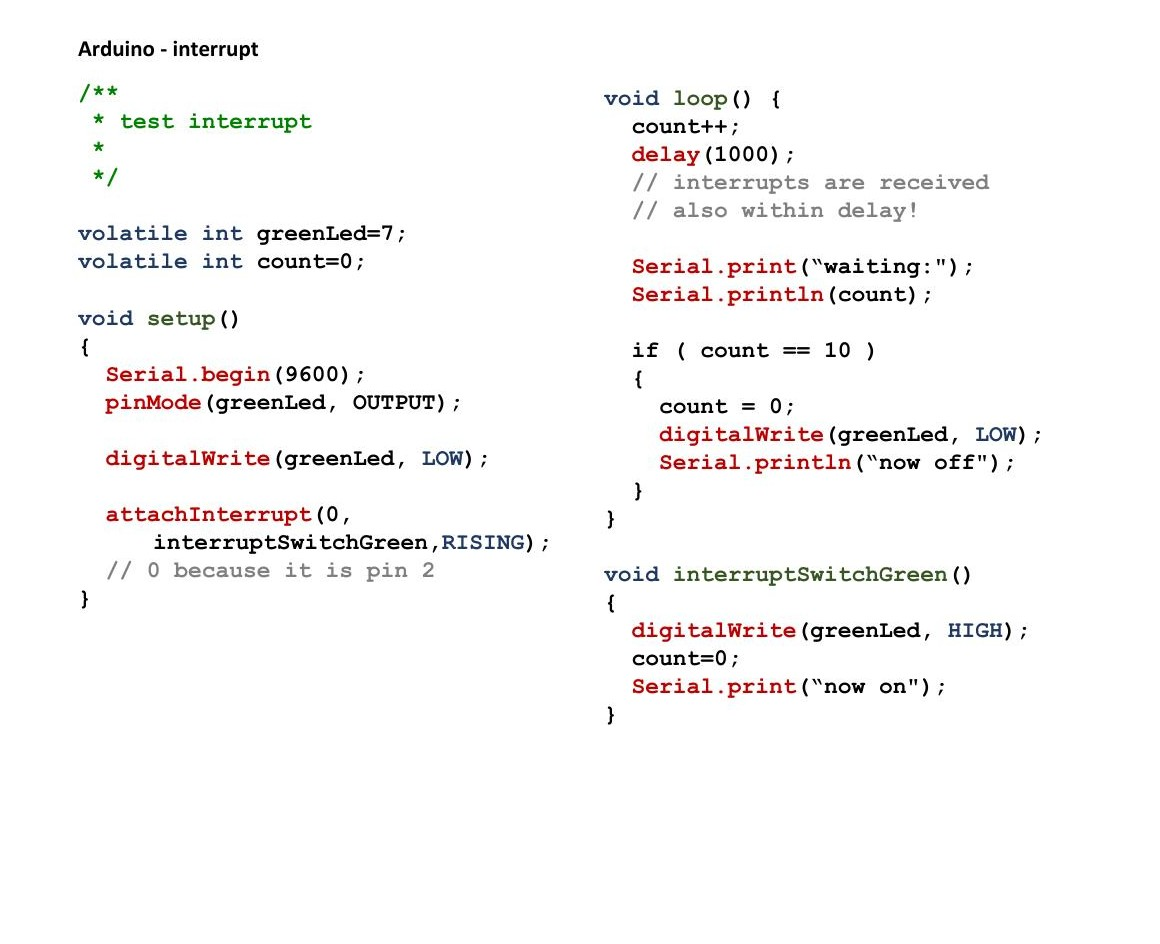
\includegraphics[keepaspectratio]{images/exam-chessa-arduino-interrupt.jpg}}
\caption{Esempio di programmazione con interrupt su Arduino:
attachInterrupt() collega il pin 2 a interruptSwitchGreen(); count viene
resettato e il LED acceso all'interrupt.}
\end{figure}

\begin{Shaded}
\begin{Highlighting}[]
\AttributeTok{volatile} \DataTypeTok{int}\NormalTok{ greenLed }\OperatorTok{=} \DecValTok{7}\OperatorTok{;}
\AttributeTok{volatile} \DataTypeTok{int}\NormalTok{ count }\OperatorTok{=} \DecValTok{0}\OperatorTok{;}

\DataTypeTok{void}\NormalTok{ setup}\OperatorTok{()} \OperatorTok{\{}
\NormalTok{  Serial}\OperatorTok{.}\NormalTok{begin}\OperatorTok{(}\DecValTok{9600}\OperatorTok{);}
\NormalTok{  pinMode}\OperatorTok{(}\NormalTok{greenLed}\OperatorTok{,}\NormalTok{ OUTPUT}\OperatorTok{);}
\NormalTok{  digitalWrite}\OperatorTok{(}\NormalTok{greenLed}\OperatorTok{,}\NormalTok{ LOW}\OperatorTok{);}
\NormalTok{  attachInterrupt}\OperatorTok{(}\DecValTok{0}\OperatorTok{,}\NormalTok{ interruptSwitchGreen}\OperatorTok{,}\NormalTok{ RISING}\OperatorTok{);} \CommentTok{// 0 = pin 2}
\OperatorTok{\}}

\DataTypeTok{void}\NormalTok{ loop}\OperatorTok{()} \OperatorTok{\{}
\NormalTok{  count}\OperatorTok{++;}
\NormalTok{  delay}\OperatorTok{(}\DecValTok{1000}\OperatorTok{);}
  \CommentTok{// Gli interrupt vengono ricevuti anche dentro delay!}
\NormalTok{  Serial}\OperatorTok{.}\NormalTok{print}\OperatorTok{(}\StringTok{"waiting:"}\OperatorTok{);}
\NormalTok{  Serial}\OperatorTok{.}\NormalTok{println}\OperatorTok{(}\NormalTok{count}\OperatorTok{);}
  \ControlFlowTok{if} \OperatorTok{(}\NormalTok{count }\OperatorTok{==} \DecValTok{10}\OperatorTok{)} \OperatorTok{\{}
\NormalTok{    count }\OperatorTok{=} \DecValTok{0}\OperatorTok{;}
\NormalTok{    digitalWrite}\OperatorTok{(}\NormalTok{greenLed}\OperatorTok{,}\NormalTok{ LOW}\OperatorTok{);}
\NormalTok{    Serial}\OperatorTok{.}\NormalTok{println}\OperatorTok{(}\StringTok{"now off"}\OperatorTok{);}
  \OperatorTok{\}}
\OperatorTok{\}}

\DataTypeTok{void}\NormalTok{ interruptSwitchGreen}\OperatorTok{()} \OperatorTok{\{}
\NormalTok{  digitalWrite}\OperatorTok{(}\NormalTok{greenLed}\OperatorTok{,}\NormalTok{ HIGH}\OperatorTok{);}
\NormalTok{  count }\OperatorTok{=} \DecValTok{0}\OperatorTok{;}
\NormalTok{  Serial}\OperatorTok{.}\NormalTok{print}\OperatorTok{(}\StringTok{"now on"}\OperatorTok{);}
\OperatorTok{\}}
\end{Highlighting}
\end{Shaded}

Arduino Uno dispone di \textbf{due pin per interrupt esterni}: INT0 (pin
2) e INT1 (pin 3).
\texttt{attachInterrupt(0,\ interruptSwitchGreen,\ RISING)} collega il
pin 2 alla funzione \texttt{interruptSwitchGreen}, eseguita
automaticamente sul fronte di salita del segnale.

\textbf{Punti chiave e regole per gli interrupt handler}: -
\texttt{delay()} \textbf{non funziona} dentro un interrupt handler -
\texttt{millis()} \textbf{non viene incrementato} dentro un interrupt
handler\\
- La variabile \texttt{count} è dichiarata \texttt{volatile}: indica al
compilatore di non ottimizzarla in registro (forza la lettura dalla
RAM), perché può essere modificata da handler fuori dal flusso normale,
garantendo la coerenza del valore. - Gli interrupt sono ricevuti
\textbf{anche durante \texttt{delay()}}: il delay non disabilita gli
interrupt, quindi l'handler può intervenire in qualsiasi momento. - I
handler devono essere \textbf{il più brevi possibile}: solo
aggiornamento di strutture dati e comandi all'HW. - \textbf{Utilizzo
tipico negli embedded IoT}: gli interrupt sono usati per ricevere dati
dal sensore (read done), notificare la fine di una trasmissione radio, o
rispondere a eventi fisici senza polling continuo, risparmiando energia.

\begin{center}\rule{0.5\linewidth}{0.5pt}\end{center}

\section{Calcolo del Duty Cycle e Gestione
Energetica}\label{calcolo-del-duty-cycle-e-gestione-energetica}

\begin{figure}
\centering
\pandocbounded{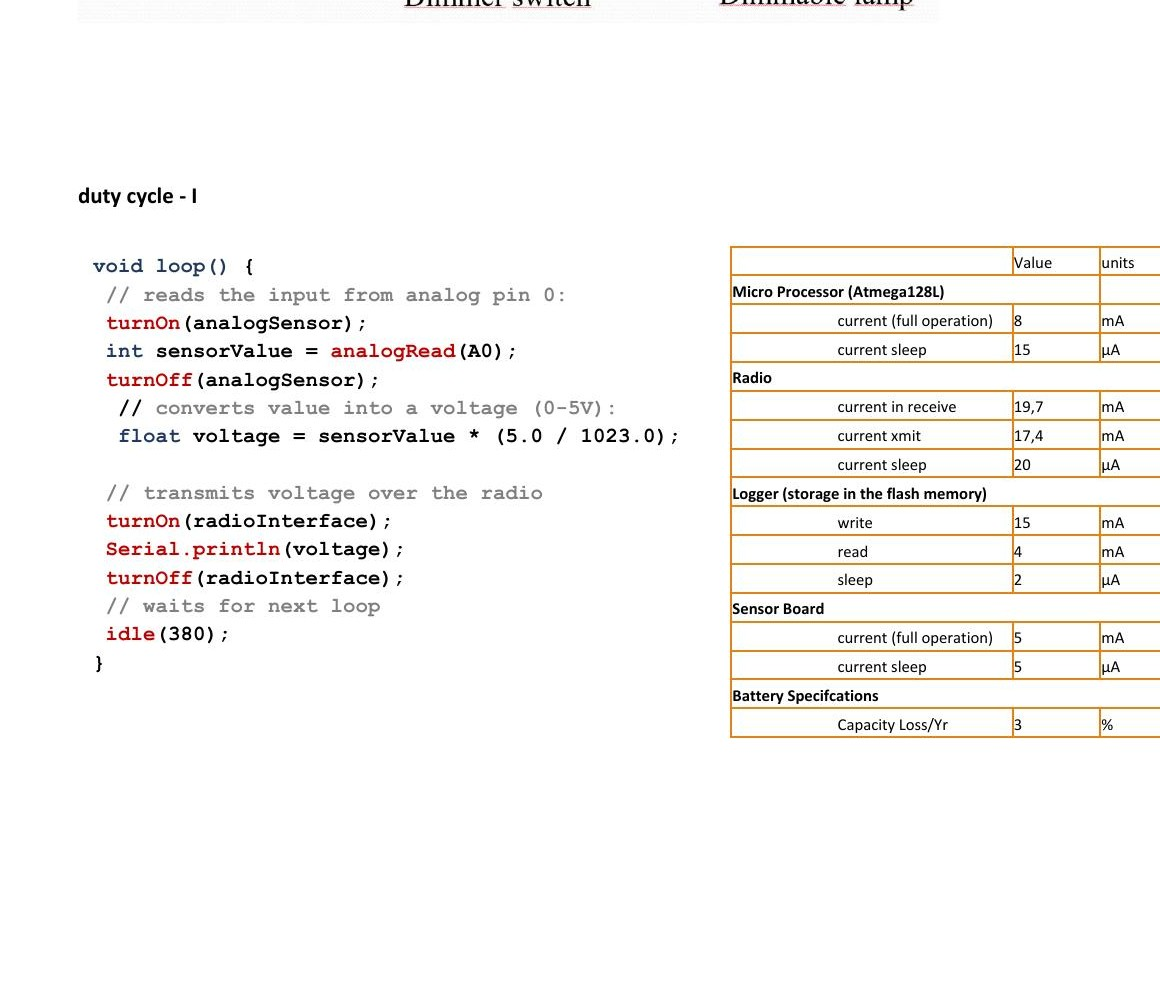
\includegraphics[keepaspectratio]{images/exam-chessa-dutycycle-code.jpg}}
\caption{Codice Arduino che implementa il duty cycling selettivo dei
componenti (sensore, radio) e tabella dei consumi in mA per componente e
stato.}
\end{figure}

Il \textbf{duty cycle} di un componente è la frazione di tempo in cui è
attivo rispetto al periodo totale. La strategia fondamentale di
risparmio energetico nei dispositivi IoT è attivare ogni componente
\textbf{solo quando strettamente necessario}.

Il codice mostra il pattern classico:

\begin{verbatim}
turnOn(analogSensor)   → sensore acceso solo durante lettura
analogRead(A0)         → lettura
turnOff(analogSensor)  → sensore spento

turnOn(radioInterface) → radio accesa solo durante trasmissione
Serial.println(voltage)
turnOff(radioInterface)

idle(380)              → MCU in sleep 380ms
\end{verbatim}

\begin{callouttip}{Calcolo del Duty Cycle}

Usando i valori della tabella (es. Tmote Sky): - Processore attivo: 8
mA, sleep: 15 μA - Radio TX: 17.4 mA, RX: 19.7 mA, sleep: 20 μA -
Sensore: 5 mA, sleep: 5 μA

Se le operazioni di sensing + TX durano \textasciitilde20 ms e il ciclo
totale è 400 ms, il duty cycle della radio è 20/400 = 5\%. La corrente
media risultante è molto inferiore alla corrente di picco, estendendo la
vita della batteria di ordini di grandezza. Il sistema è attivo solo per
circa il 5\% del tempo.

\end{callouttip}

\subsection{Impatto sulla Vita della
Batteria}\label{impatto-sulla-vita-della-batteria}

\begin{figure}
\centering
\pandocbounded{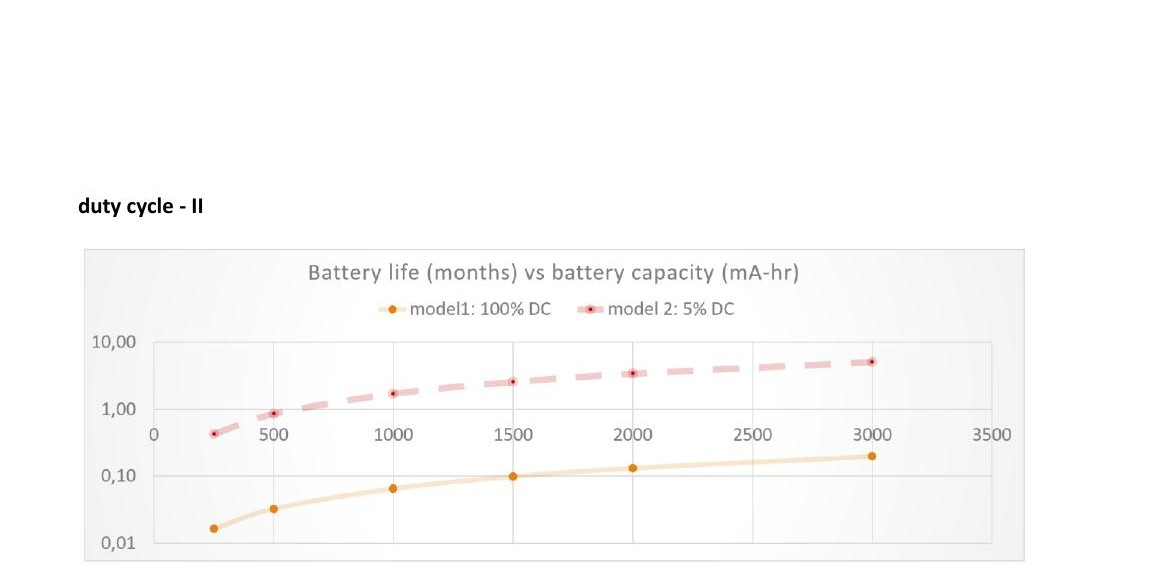
\includegraphics[keepaspectratio]{images/exam-chessa-dutycycle-graph.jpg}}
\caption{Grafico log-log: vita della batteria (mesi) vs capacità della
batteria (mAh) per duty cycle 100\% (model1) e 5\% (model2).}
\end{figure}

Il grafico mostra l'impatto del duty cycle sulla vita della batteria in
scala logaritmica. Due modelli a confronto:

\begin{itemize}
\tightlist
\item
  \textbf{Model 1 (100\% DC)}: il dispositivo è sempre attivo. La vita
  della batteria scala linearmente con la capacità ma rimane nell'ordine
  dei mesi (0.01--0.3 mesi per capacità 500--3000 mAh).
\item
  \textbf{Model 2 (5\% DC)}: il dispositivo è attivo solo il 5\% del
  tempo. La vita si estende di un fattore \textasciitilde20: con la
  stessa batteria, si passa da 0.1 a circa 2--8 mesi.
\end{itemize}

La scala logaritmica rivela che la relazione vita-capacità non è
lineare: il duty cycle agisce moltiplicativamente. Ridurre il duty cycle
da 100\% a 5\% equivale a moltiplicare la capacità effettiva della
batteria per 20.

\textbf{Conclusione progettuale}: per applicazioni IoT con autonomia di
anni, ridurre il duty cycle è molto più efficace che aumentare la
capacità della batteria. Una batteria da 3000 mAh a 5\% DC dura circa 8
mesi; per durare anni si deve abbassare ulteriormente il duty cycle o
usare energy harvesting. La perdita di capacità della batteria del
3\%/anno indica che anche con battery standby c'è un degrado nel tempo.

\newpage

\chapter{Energy Harvesting IoT}\label{energy-harvesting-iot}

Il problema di fondo dei dispositivi IoT è energetico: alimentarli con
una batteria di capacità finita costringe a scegliere tra prestazioni e
durata. Una batteria grande permette lunga vita, ma aumenta dimensioni,
peso e costo; un processore a basso consumo estende la vita ma limita
potenza di calcolo e portata radio. L'\textbf{energy harvesting}
(raccolta di energia) rappresenta un'alternativa strutturale: invece di
ottimizzare il consumo, si raccoglie energia dall'ambiente e si elimina
--- o si riduce drasticamente --- il vincolo della batteria finita.

\section{Architetture di harvesting e Concetto di Energy
Neutrality}\label{architetture-di-harvesting-e-concetto-di-energy-neutrality}

\subsection{Harvest-Use vs
Harvest-Store-Use}\label{harvest-use-vs-harvest-store-use}

\textbf{Harvest-Use}: l'energia è raccolta e consumata istantaneamente.
Non esiste un buffer. Il dispositivo funziona solo se
\(P_s(t) \geq P_c(t)\) (potenza sorgente ≥ potenza consumata). Se la
sorgente produce meno del necessario il dispositivo si spegne; se
produce di più l'eccesso va perduto. Esempi: mulini ad acqua, tag RFID
passivi.

\textbf{Harvest-Store-Use}: un buffer energetico (batteria ricaricabile
o supercapacitore) disaccoppia temporalmente produzione e consumo.
L'energia in eccesso (\(P_s > P_c\)) viene accumulata nel buffer;
l'energia in difetto (\(P_c > P_s\)) viene prelevata dal buffer. Un
buffer ideale ha capacità infinita ed efficienza \(\eta = 1\). Un buffer
reale ha capacità massima \(B_{max}\), efficienza \(\eta < 1\), e una
potenza di leakage \(P_{leak}\).

\subsection{Concetto di Energy
Neutrality}\label{concetto-di-energy-neutrality}

Un dispositivo è \textbf{energy neutral} se, in qualsiasi intervallo di
tempo, l'energia consumata non supera l'energia raccolta (più la carica
iniziale del buffer):

\[\int_0^T P_c(t)\,dt \leq \int_0^T P_s(t)\,dt + B_0 \qquad \forall T\]

Il raggiungimento dell'energy neutrality richiede di adattare il carico
in base alla disponibilità energetica prevista --- obiettivo del
problema di Kansal.

\section{Analisi Grafica della Potenza e Neutralità
Energetica}\label{analisi-grafica-della-potenza-e-neutralituxe0-energetica}

\begin{figure}
\centering
\pandocbounded{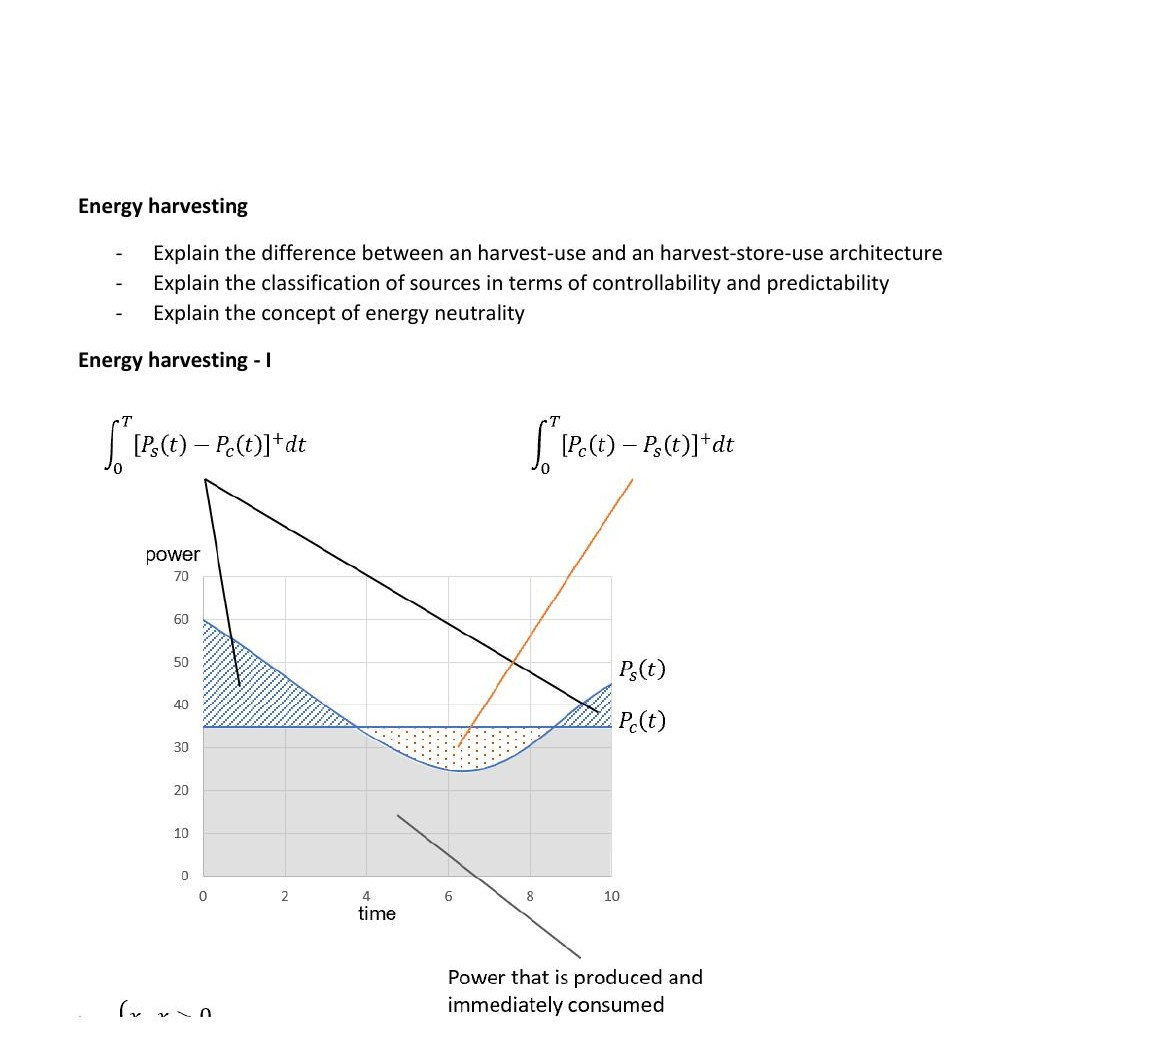
\includegraphics[keepaspectratio]{images/exam-chessa-energy-neutrality-graph.jpg}}
\caption{Grafico potenza/tempo: l'area tratteggiata in blu (Ps
\textgreater{} Pc) è l'energia raccolta e accumulata nel buffer; l'area
punteggiata (Pc \textgreater{} Ps) è l'energia prelevata dal buffer. La
retta arancione mostra l'energia immediatamente consumata (Pc=Ps).}
\end{figure}

Il grafico mostra due curve di potenza in funzione del tempo: -
\(P_s(t)\): potenza prodotta dall'energy harvester (curva decrescente).
- \(P_c(t)\): potenza consumata dal dispositivo (curva a forma di U).

Le due aree rappresentano:

\[\int_0^T [P_s(t) - P_c(t)]^+ dt\]

Area in blu (Ps \textgreater{} Pc): energia prodotta in eccesso →
accumulata nel buffer. Il buffer si carica.

\[\int_0^T [P_c(t) - P_s(t)]^+ dt\]

Area punteggiata (Pc \textgreater{} Ps): il consumo supera la produzione
→ energia prelevata dal buffer. Il buffer si scarica.

La retta arancione indica la zona in cui \(P_s = P_c\): energia prodotta
e immediatamente consumata, senza passare dal buffer. Il sistema è
energy neutral se la prima integrale ≥ seconda integrale su tutto
l'orizzonte temporale considerato.

\section{Classificazione delle
Sorgenti}\label{classificazione-delle-sorgenti}

Le sorgenti si classificano su due assi:

\textbf{Controllabilità}: - \emph{Completamente controllabile}: energia
disponibile su richiesta (torcia shake-to-power, sorgenti RF dedicate).
- \emph{Parzialmente controllabile}: influenzabile ma non deterministica
(RFID in ambiente RF non uniforme). - \emph{Non controllabile}: raccolta
solo quando disponibile (sole, vento, calore ambientale).

\textbf{Prevedibilità} (per le sorgenti non controllabili): -
\emph{Prevedibile}: esistono modelli affidabili (sole: ciclo
giorno/notte + stagioni + meteo). - \emph{Non prevedibile}: nessun
modello affidabile (vibrazioni da terremoti).

\section{Misurare la carica della
batteria}\label{misurare-la-carica-della-batteria}

Tutte le tecniche di power management richiedono informazioni fresche
sulla carica attuale della batteria e sulla produzione energetica.
Entrambe sono quantità non direttamente osservabili e devono essere
stimate.

\subsection{Stima Stato di Carica tramite
ADC}\label{stima-stato-di-carica-tramite-adc}

\begin{figure}
\centering
\pandocbounded{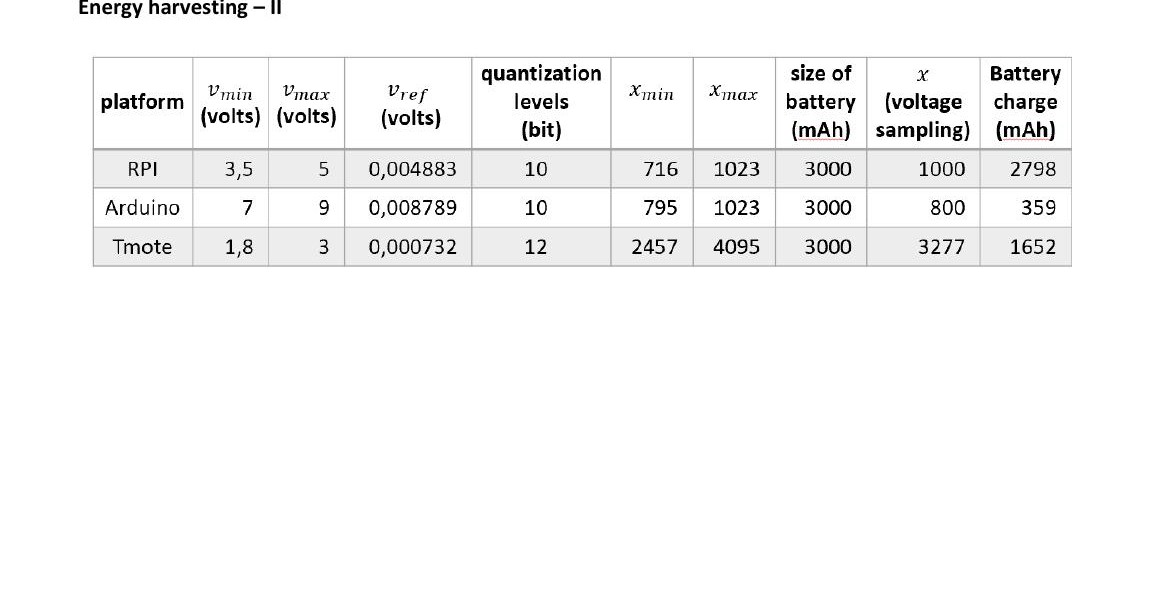
\includegraphics[keepaspectratio]{images/exam-chessa-energy-harvesting-table.jpg}}
\caption{Tabella con parametri di batteria per tre piattaforme (RPI,
Arduino, Tmote): tensioni min/max/ref, livelli di quantizzazione,
xmin/xmax e stima Battery charge.}
\end{figure}

La tabella mostra come misurare lo \textbf{stato di carica} (SoC) di una
batteria attraverso la sua tensione terminale, per tre piattaforme
hardware. L'idea è che la tensione ai terminali di una batteria è
approssimabile come monotona (e in molti tratti lineare) rispetto alla
carica residua.

Le colonne chiave: - \(v_{min}\), \(v_{max}\): range operativo della
batteria (es. Arduino: 7--9 V). - \(v_{ref}\): risoluzione della
quantizzazione ADC (es. Arduino: 0.008789 V per LSB). -
\textbf{quantization levels (bit)}: risoluzione dell'ADC (10 o 12 bit).
- \(x_{min}\), \(x_{max}\): valori ADC corrispondenti a \(v_{min}\) e
\(v_{max}\). - \textbf{Battery charge (mAh)}: capacità totale della
batteria stimata.

Campionando la tensione tramite ADC e mappando il valore digitale \(x\)
nell'intervallo \([x_{min}, x_{max}]\), si ottiene una stima lineare
della carica rimanente:

\[\text{SoC} \approx \frac{x - x_{min}}{x_{max} - x_{min}} \times B_{cap}\]
\[B = B_{min} + \frac{B_{max} - B_{min}}{x_{max} - x_{min}}(x - x_{min})\]

Questa stima è utile per il task scheduler: sa quanta energia ha
disponibile e può pianificare i task di conseguenza.

\newpage

\chapter{Kansal Problem e Energy
Neutrality}\label{kansal-problem-e-energy-neutrality}

\section{Il Problema di Kansal: Energy Neutrality nei Sistemi
IoT}\label{il-problema-di-kansal-energy-neutrality-nei-sistemi-iot}

Il problema di \textbf{energy management} per dispositivi IoT alimentati
da sorgenti rinnovabili è intrinsecamente legato alla natura della
sorgente di energia. Kansal considera il caso di sorgenti
\textbf{prevedibili ma non controllabili}: fonti come l'energia solare
sono soggette a variazioni giornaliere e stagionali, ma il loro
andamento nel tempo può essere stimato con buona precisione.

L'obiettivo del power management è triplice: - mantenere il sistema
\textbf{energy neutral}, cioè fare in modo che la batteria non si
esaurisca mai; - \textbf{evitare che il dispositivo si spenga} prima del
prossimo ciclo di ricarica; - \textbf{massimizzare le prestazioni} del
nodo, ossia la sua utility.

L'approccio consiste nel tener conto del livello attuale e atteso della
batteria, modulare dinamicamente le prestazioni del dispositivo (e
quindi il carico energetico), garantendo che il dispositivo non scenda
sotto le performance minime.

\subsection{Approccio Kansal all'Energy
Neutrality}\label{approccio-kansal-allenergy-neutrality}

\begin{figure}
\centering
\pandocbounded{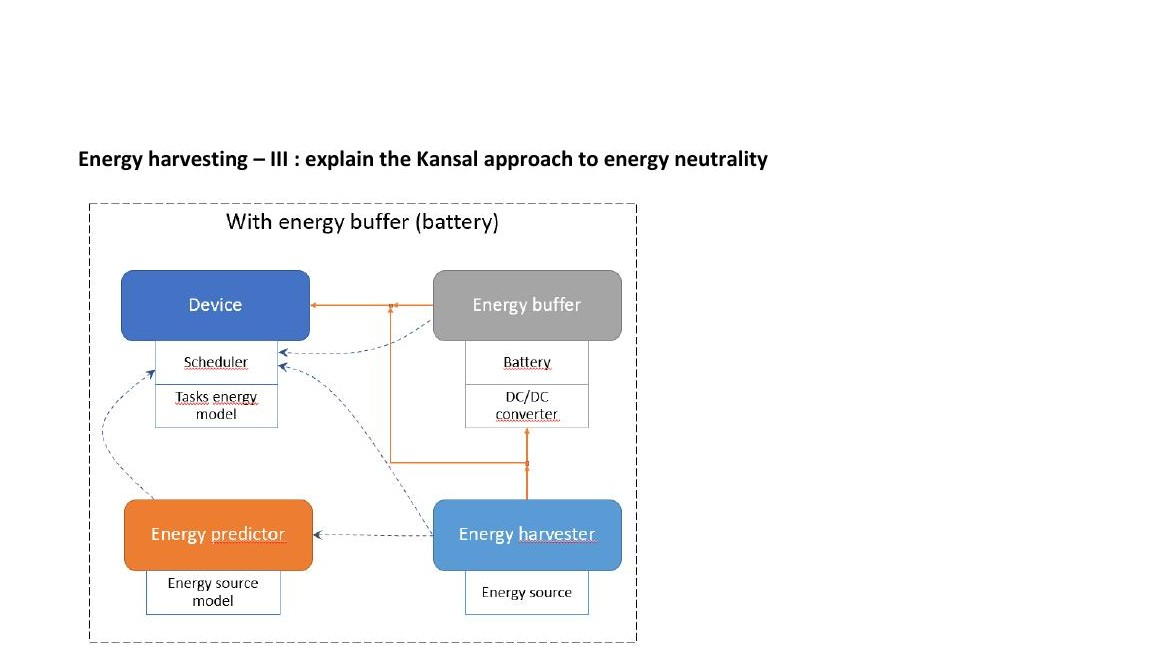
\includegraphics[keepaspectratio]{images/exam-chessa-kansal-system.jpg}}
\caption{Sistema Kansal: il Device (con Scheduler e Tasks energy model)
è alimentato dall'Energy buffer (Battery + DC/DC converter), rifornito
dall'Energy harvester. L'Energy predictor stima la disponibilità futura
e informa lo Scheduler.}
\end{figure}

L'approccio di \textbf{Kansal} all'energy neutrality mira a massimizzare
le prestazioni del dispositivo garantendo al contempo che la batteria
non si scarichi mai completamente (energy neutral operation). L'idea è
pianificare dinamicamente il duty cycle del dispositivo slot per slot,
sfruttando previsioni sulla produzione futura.

Il sistema è composto da: - \textbf{Energy harvester}: raccoglie energia
dalla sorgente (es. pannello solare). - \textbf{Energy buffer (Battery +
DC/DC converter)}: accumula l'energia raccolta e la cede al dispositivo
quando necessario. - \textbf{Energy predictor} (con Energy source
model): stima la quantità di energia che sarà disponibile nel futuro (ad
es. usando previsioni meteo per un pannello solare). - \textbf{Device}
con \textbf{Scheduler} (e Tasks energy model): pianifica quali task
eseguire e a quale frequenza, basandosi sia sullo stato attuale della
batteria sia sulla predizione energetica futura.

\textbf{Idea centrale}: adattare il carico (\(P_c\)) alla disponibilità
energetica prevista. Se le previsioni indicano un giorno soleggiato → il
dispositivo può aumentare la frequenza di campionamento. Se le
previsioni indicano bassa produzione → il dispositivo riduce l'attività.

\textbf{Condizione di energy neutrality di Kansal}:
\[B_T = B_0 + \eta \int_0^T [P_s - P_c]^+ dt - \int_0^T [P_c - P_s]^+ dt \geq B_{min} \quad \forall T\]

Il Kansal problem è quindi un problema di ottimizzazione: massimizzare
le prestazioni (es. frequenza di campionamento) soggetto al vincolo di
energy neutrality.

\begin{center}\rule{0.5\linewidth}{0.5pt}\end{center}

\section{Modello Task-Based per l'Energy
Neutrality}\label{modello-task-based-per-lenergy-neutrality}

Kansal modella il carico tramite duty cycle, ma le applicazioni IoT
reali sono più complesse. Un'applicazione tipica esegue 4 fasi in ciclo:
\textbf{Sensing → Storing → Processing → Transmitting}. Ciascuna fase
può avere implementazioni alternative con diversi trade-off
energia/performance.

Si chiama \textbf{task} un'implementazione specifica dell'applicazione
sul dispositivo IoT. Un dispositivo ha \(n\) task alternative, ciascuna
con costo energetico \(c_j\) e utility \(u_j\).

\begin{figure}
\centering
\pandocbounded{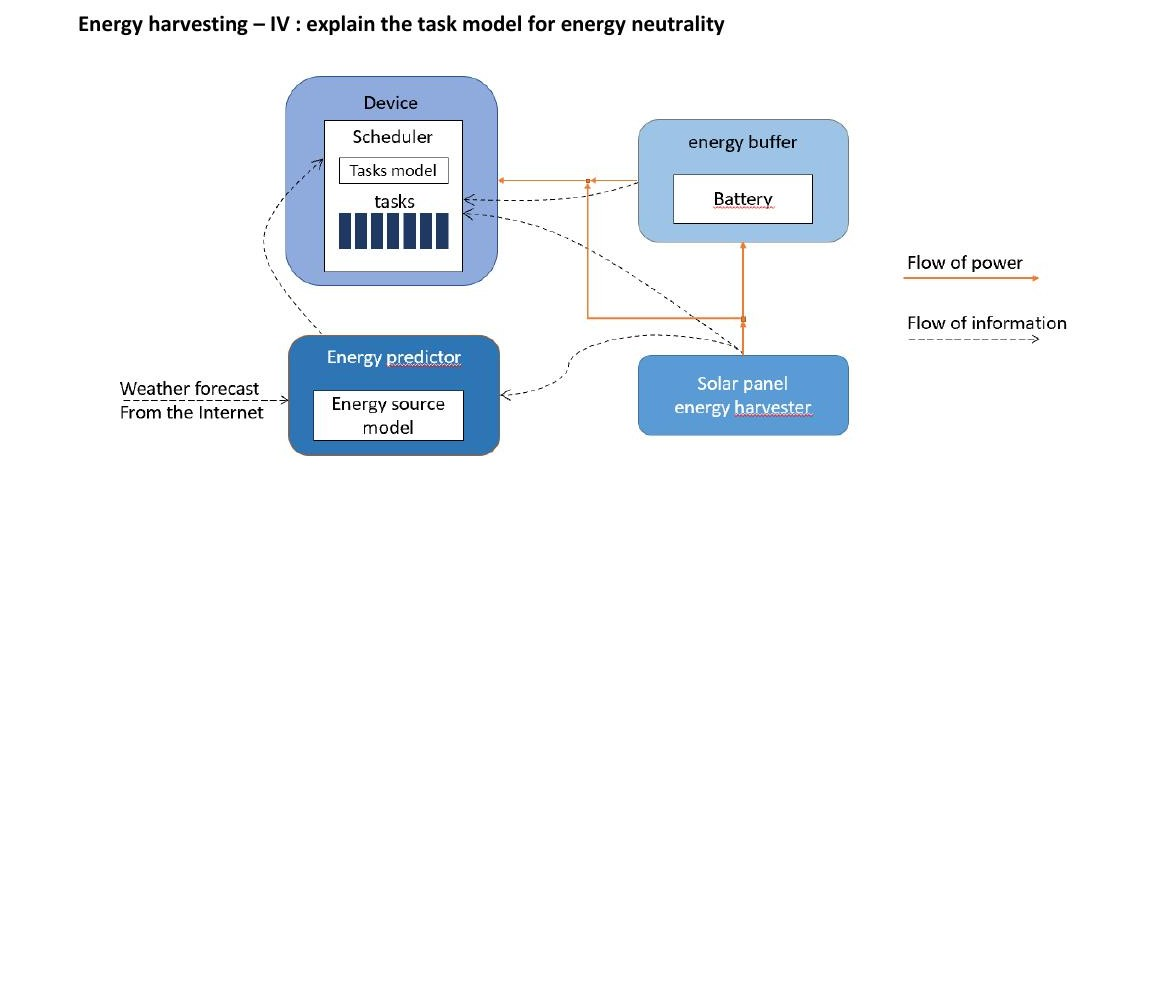
\includegraphics[keepaspectratio]{images/exam-chessa-kansal-taskmodel.jpg}}
\caption{Task model: lo Scheduler pianifica i task in base al Tasks
model (energia per task) e alle previsioni energetiche dell'Energy
predictor (alimentato da weather forecast e da un Solar panel harvester
collegato alla Battery).}
\end{figure}

Lo schema espande il sistema Kansal con il dettaglio del \textbf{task
model}. Rispetto allo schema base, qui è esplicitato il ruolo delle
previsioni meteorologiche esterne.

\textbf{Componenti}: - \textbf{Tasks model}: specifica il costo
energetico di ogni task (es. campionamento = X mJ, trasmissione = Y mJ).
Lo Scheduler usa questo modello per stimare quanta energia consumerà
ogni operazione. - \textbf{Scheduler}: dato il livello attuale della
batteria e la previsione di energia futura, decide: - Quali task
eseguire nel prossimo periodo. - A quale frequenza/duty cycle eseguirli.
- Obiettivo: massimizzare la qualità del servizio senza violare l'energy
neutrality. - \textbf{Energy predictor + Energy source model}: riceve
dati dal weather forecast (Internet) e dalle misurazioni del pannello
solare per costruire un modello predittivo della produzione energetica
futura. - \textbf{Solar panel energy harvester → Battery}: flusso di
potenza fisico; informazioni di stato comunicano il livello di carica
allo Scheduler.

Lo scheduler assegna esattamente un task per slot, ottimizzando
l'utility complessiva e rispettando i vincoli di batteria e la
neutralità energetica di fine giornata.

\newpage

\chapter{Interoperabilità e Standard
nell'IoT}\label{interoperabilituxe0-e-standard-nelliot}

Il concetto di \textbf{interoperabilità} rappresenta una delle sfide
cruciali nello sviluppo dell'Internet of Things. Implementare una
soluzione IoT ``dal basso'', ovvero dal livello fisico fino
all'applicazione, non costituisce di per sé un problema tecnico
insormontabile; tuttavia, questo approccio porta spesso alla creazione
di quelli che vengono definiti \emph{vertical silos}.

\begin{figure}
\centering
\pandocbounded{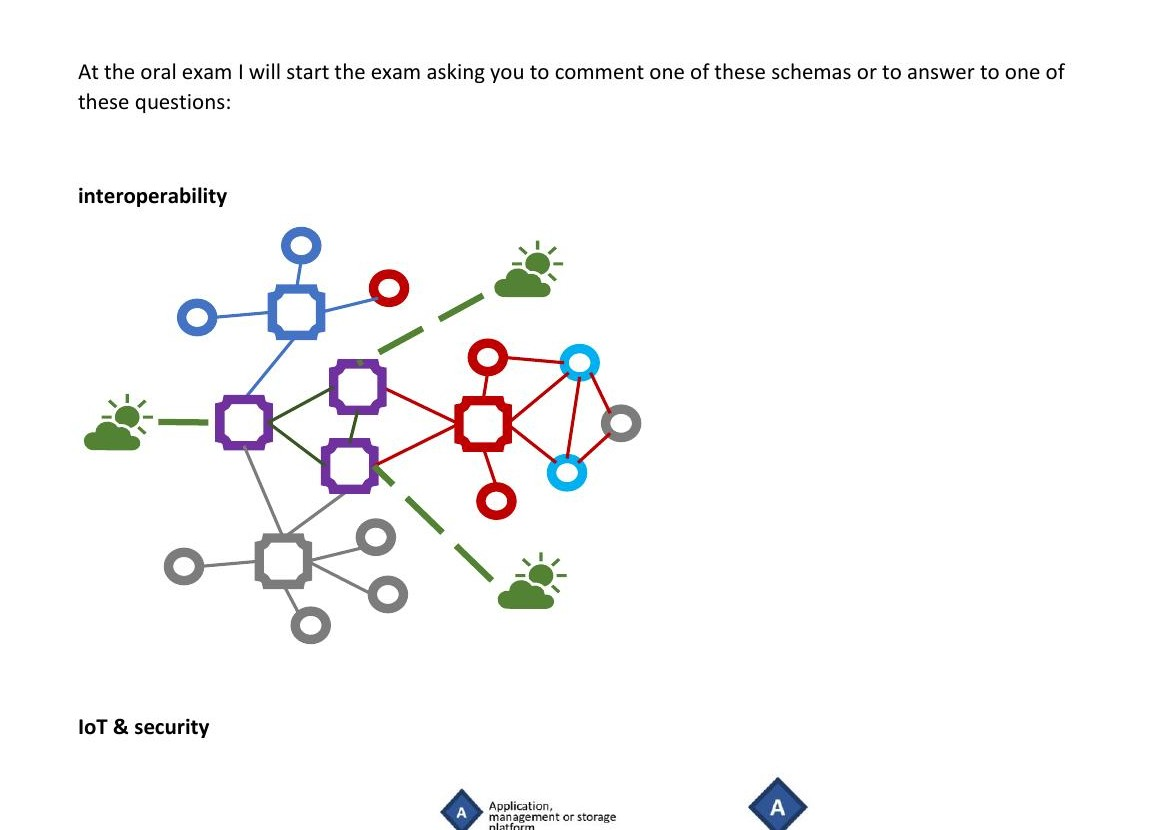
\includegraphics[keepaspectratio]{images/exam-chessa-interoperability.jpg}}
\caption{Rete IoT eterogenea: dispositivi di produttori diversi (colori
diversi) comunicano attraverso gateway di integrazione.}
\end{figure}

Lo schema mostra una rete in cui dispositivi appartenenti a ecosistemi
diversi devono comunicare tra loro. Il problema fondamentale è proprio
l'\textbf{interoperabilità}.

\begin{calloutdefinition}{Vertical Silos}

In questo modello, una soluzione funziona esclusivamente all'interno del
proprio ecosistema: i dispositivi proprietari comunicano solo con
l'infrastruttura dello stesso fornitore, rendendo incompatibili i
prodotti di terze parti.

\end{calloutdefinition}

Questa strategia di design è spesso intenzionale e risponde a un modello
di business basato sul \emph{vendor lock-in}.

\begin{calloutdefinition}{Vendor Lock-in}

La pratica di ``ingabbiare'' il cliente con l'obiettivo di prevenire
l'utilizzo di componenti di altri produttori e imporre costi elevati per
l'eventuale migrazione verso soluzioni alternative. Tale migrazione
comporta spesso la completa riprogettazione e il dispiegamento di un
nuovo sistema, con il rischio di entrare semplicemente in un altro
silos.

\end{calloutdefinition}

Storicamente, il problema dell'interoperabilità risiedeva principalmente
a livello hardware, ma nell'IoT moderno la questione si è spostata
prevalentemente a livello software. La soluzione universalmente
riconosciuta per mitigare queste barriere è l'introduzione e l'adozione
di \textbf{standard} condivisi.

\section{La Necessità e la Complessità degli
Standard}\label{la-necessituxe0-e-la-complessituxe0-degli-standard}

Gli standard nascono dalla necessità di ridurre i costi di sviluppo
tecnologico attraverso accordi tra diversi produttori, in un regime di
\textbf{coopetition} (cooperazione tra competitor). Solitamente, la
standardizzazione avviene quando una tecnologia diventa matura.

Tuttavia, la proliferazione degli standard (come Wi-Fi, ZigBee,
Bluetooth) ha spostato il problema dell'interoperabilità ai livelli
middleware e applicativo. Oggi esistono numerosi protocolli di livello
applicativo (MQTT, CoAP, LWM2M, ecc.), creando una situazione in cui
l'incompatibilità non è solo tra silos verticali, ma anche tra standard
differenti.

Per gestire questa eterogeneità si ricorre agli
\textbf{Application-level gateway}. Questi dispositivi non si limitano a
tradurre protocolli di basso livello: mappano comportamenti applicativi
differenti l'uno nell'altro, operando come interpreti semantici tra
ecosistemi incompatibili.

\section{Configurazioni di
Integrazione}\label{configurazioni-di-integrazione}

Le architetture IoT possono assumere configurazioni molto diverse in
base all'omogeneità dei dispositivi e dei protocolli coinvolti. La
tabella seguente riassume i quattro tipi principali:

{\def\LTcaptype{none} % do not increment counter
\begin{longtable}[]{@{}
  >{\raggedright\arraybackslash}p{(\linewidth - 6\tabcolsep) * \real{0.1176}}
  >{\raggedright\arraybackslash}p{(\linewidth - 6\tabcolsep) * \real{0.2157}}
  >{\raggedright\arraybackslash}p{(\linewidth - 6\tabcolsep) * \real{0.2353}}
  >{\raggedright\arraybackslash}p{(\linewidth - 6\tabcolsep) * \real{0.4314}}@{}}
\toprule\noalign{}
\begin{minipage}[b]{\linewidth}\raggedright
Tipo
\end{minipage} & \begin{minipage}[b]{\linewidth}\raggedright
Fornitore
\end{minipage} & \begin{minipage}[b]{\linewidth}\raggedright
Protocollo
\end{minipage} & \begin{minipage}[b]{\linewidth}\raggedright
Necessità di gateway
\end{minipage} \\
\midrule\noalign{}
\endhead
\bottomrule\noalign{}
\endlastfoot
A & Unico & Unico & No \\
B & Multiplo & Unico (condiviso) & No o minimale \\
C & Multiplo & Diversi & Sì --- Integration Gateway per la traduzione \\
D & Multiplo & Eterogenei e distribuiti & Sì --- gateway multipli con
mappature complesse \\
\end{longtable}
}

Al crescere della complessità, dal Tipo A al Tipo D, il gateway di
integrazione deve gestire un numero esponenziale di mappature tra
protocolli allo stesso livello. La sfida non è solo tecnica ma
organizzativa: ogni nuovo fornitore o protocollo aggiunto alla rete
moltiplica le combinazioni da gestire.

\begin{center}\rule{0.5\linewidth}{0.5pt}\end{center}

\section{Sicurezza nell'IoT}\label{sicurezza-nelliot}

\begin{figure}
\centering
\pandocbounded{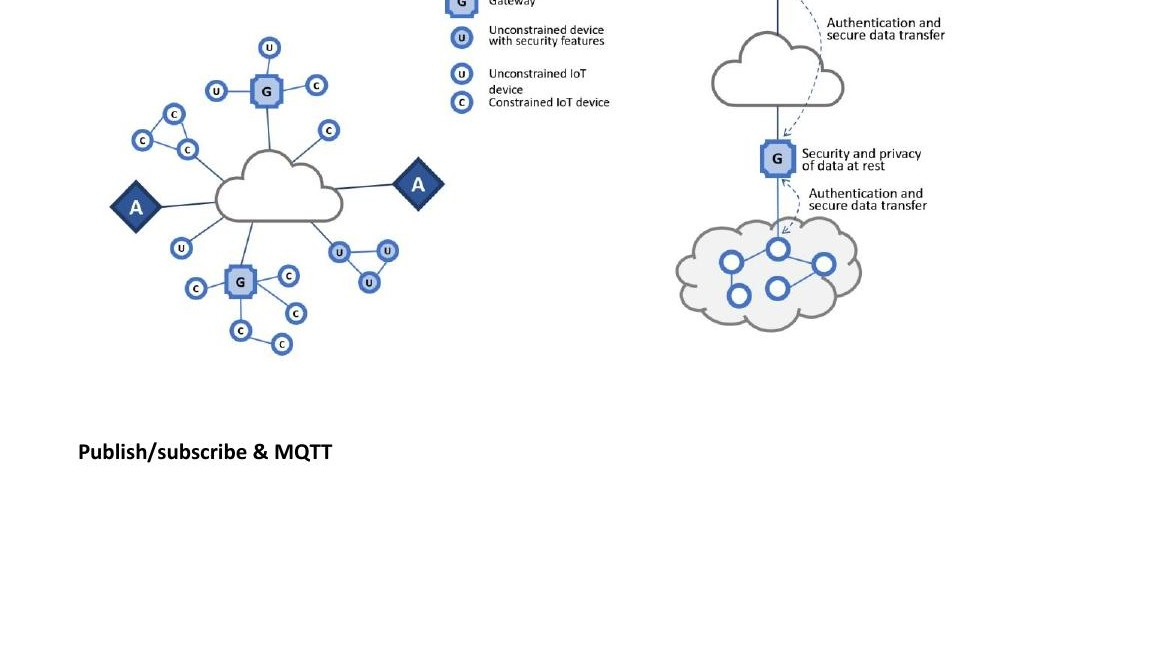
\includegraphics[keepaspectratio]{images/exam-chessa-iot-security.jpg}}
\caption{Architettura di sicurezza IoT: dispositivi vincolati (C),
gateway (G), applicazioni (A) e relative misure di sicurezza per ogni
livello.}
\end{figure}

Lo schema mostra un'architettura IoT a strati in cui la sicurezza deve
essere garantita a ogni livello: tra dispositivi periferici e gateway
(autenticazione + trasferimento sicuro), e tra gateway e
cloud/applicazione (sicurezza dei dati a riposo + autenticazione).

La sicurezza nei sistemi cyber-fisici e nell'IoT ha raggiunto un punto
di crisi. A differenza dei sistemi IT tradizionali, i dispositivi IoT
sono spesso sistemi embedded economici, prodotti con forti incentivi a
ridurre costi e tempi di immissione sul mercato (\emph{Time-to-Market}),
a discapito della sicurezza. La conseguenza sono centinaia di milioni di
dispositivi vulnerabili, privi di meccanismi di patching efficaci.

Le conseguenze variano dall'inserimento di dati falsi nella rete alla
compromissione delle operazioni fisiche.

\section{Requisiti di Sicurezza secondo ITU-T
Y.2066}\label{requisiti-di-sicurezza-secondo-itu-t-y.2066}

La raccomandazione \textbf{Y.2066} dell'ITU-T identifica i requisiti
fondamentali per la sicurezza IoT organizzandoli in tre aree concettuali
distinte:

\begin{enumerate}
\def\labelenumi{\arabic{enumi}.}
\tightlist
\item
  \textbf{Sicurezza della comunicazione}: garantire la riservatezza e
  l'integrità dei dati in transito o il trasferimento tra dispositivi e
  piattaforme.
\item
  \textbf{Sicurezza della gestione dei dati}: proteggere riservatezza e
  integrità quando i dati sono archiviati o elaborati (\emph{data at
  rest}).
\item
  \textbf{Sicurezza della fornitura del servizio}: prevenire accessi non
  autorizzati ai servizi e proteggere le informazioni private degli
  utenti.
\end{enumerate}

A questi si aggiungono l'\textbf{autenticazione mutua} (entrambe le
parti si verificano reciprocamente) e la capacità di audit di sicurezza.

\section{Il Ruolo del Gateway nella
Sicurezza}\label{il-ruolo-del-gateway-nella-sicurezza}

In un'architettura IoT, il gateway agisce spesso come punto centrale di
applicazione delle policy di sicurezza. - Gestisce identificazione e
autenticazione di ogni dispositivo connesso. - Protegge la privacy dei
dispositivi periferici. - Supporta manutenzione, aggiornamento firmware
e autodiagnosi remota. - Applica policy di configurazione dinamiche.

\begin{calloutwarning}{Dispositivi vincolati e limiti di sicurezza}

I \textbf{dispositivi vincolati} (\emph{constrained devices}) pongono
ostacoli concreti, spesso non disponendo di hardware crittografico
dedicato, rendendo impraticabile la cifratura dei dati archiviati. Con
la diffusione del \emph{Massive IoT}, la privacy diventa una criticità
per l'enorme mole di dati sensibili raccolti.

\end{calloutwarning}

\newpage

\chapter{Fondamenti dell'IoT e Architettura del Protocollo
MQTT}\label{fondamenti-delliot-e-architettura-del-protocollo-mqtt}

\section{Introduzione al Protocollo
MQTT}\label{introduzione-al-protocollo-mqtt}

\begin{calloutdefinition}{MQTT}

\textbf{MQTT} (\emph{Message Queuing Telemetry Transport}) è un
protocollo di messaggistica leggero di tipo publish/subscribe,
progettato per ambienti con risorse limitate e connettività instabile.

\end{calloutdefinition}

MQTT è stato creato nel 1999. La sua leggerezza si manifesta nel code
footprint ridotto, basso consumo di banda e overhead minimo. Dal punto
di vista architetturale, MQTT si appoggia su TCP/IP (porta 1883 in
chiaro, 8883 con SSL/TLS).

L'infrastruttura MQTT concentra volutamente la complessità sul lato
server (il broker), mantenendo l'implementazione client estremamente
semplice. È \emph{data agnostic} (il payload può essere binario, testo,
JSON o XML).

\begin{center}\rule{0.5\linewidth}{0.5pt}\end{center}

\section{Il Paradigma Publish /
Subscribe}\label{il-paradigma-publish-subscribe}

\begin{figure}
\centering
\pandocbounded{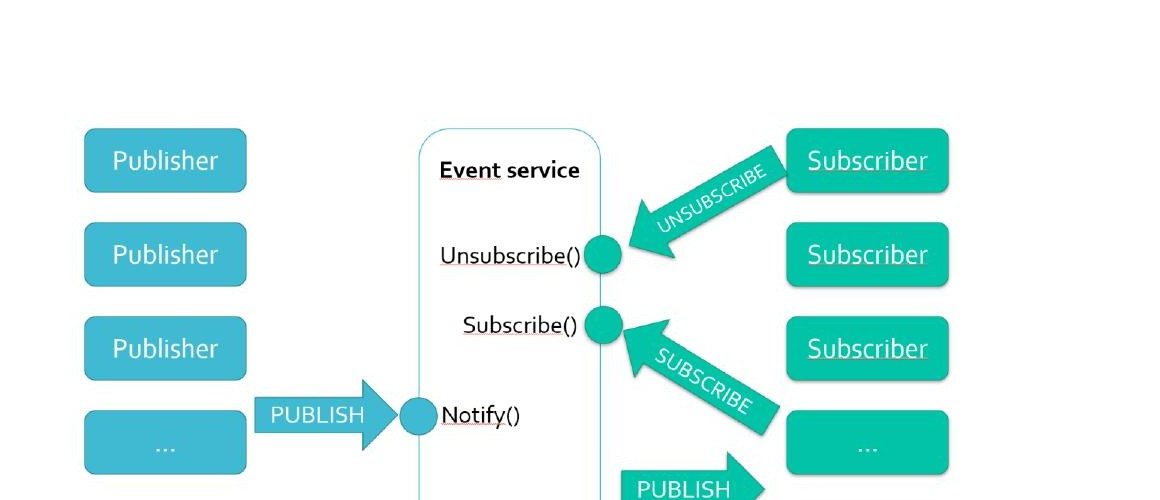
\includegraphics[keepaspectratio]{images/exam-chessa-mqtt-pubsub.jpg}}
\caption{Il paradigma publish/subscribe: i publisher inviano messaggi al
broker tramite PUBLISH; i subscriber si registrano (SUBSCRIBE) e
ricevono notifiche (PUBLISH dal broker); possono anche disdire
(UNSUBSCRIBE).}
\end{figure}

A differenza del rigido paradigma client/server, il pub/sub implementa
uno schema di interazione \emph{loosely coupled}. Gli attori sono due: i
\textbf{publisher} (pubblicatori) e i \textbf{subscriber}
(sottoscrittori), che agiscono entrambi come client senza essere a
conoscenza dell'esistenza reciproca. I publisher producono eventi
interagendo unicamente con il broker; i subscriber esprimono il proprio
interesse verso specifici topic e ricevono notifiche.

\begin{callouttip}{Pub/Sub e i tre disaccoppiamenti}

Il paradigma \textbf{publish/subscribe} introduce tre forme di
\emph{decoupling} che lo rendono ideale per l'IoT: - \textbf{Space
decoupling}: publisher e subscriber non si conoscono, non condividono IP
né porta. - \textbf{Time decoupling}: non devono essere operativi
contemporaneamente. - \textbf{Synchronization decoupling}: le operazioni
sui client non vengono bloccate durante publish o receive.

\end{callouttip}

Il \textbf{broker} è il server dell'infrastruttura: riceve tutti i
messaggi, li filtra per topic, li distribuisce ai subscriber
interessati. Le operazioni fondamentali sono quattro: \emph{Publish},
\emph{Subscribe}, \emph{Notify}, \emph{Unsubscribe}.

\begin{center}\rule{0.5\linewidth}{0.5pt}\end{center}

\section{Il Modello MQTT: Connessione e Flusso
Operativo}\label{il-modello-mqtt-connessione-e-flusso-operativo}

MQTT adotta il paradigma pub/sub con filtraggio basato su
\textbf{topic}.

\subsection{L'Instaurazione della
Connessione}\label{linstaurazione-della-connessione}

L'interazione inizia con un pacchetto \textbf{CONNECT}, contenente
parametri come: Client ID, Clean Session, Username/Password, Will flags
e KeepAlive. Il broker risponde con un \textbf{CONNACK}.

\subsection{Gestione e Best Practices dei
Topic}\label{gestione-e-best-practices-dei-topic}

Il broker usa il \textbf{filtraggio basato su topic} (topic-based
filtering). I topic sono stringhe gerarchiche separate da \texttt{/}
(es. \texttt{home/firstfloor/bedroom/temperature}). I subscriber possono
usare wildcard: - \textbf{\texttt{+}}: sostituisce un singolo livello
(es. \texttt{home/+/temperature}). - \textbf{\texttt{\#}}: sostituisce
tutti i livelli successivi (es. \texttt{home/\#}).

Il broker non ispeziona il payload, consentendo cifratura end-to-end.

\subsection{Pubblicazione e Struttura dei
Messaggi}\label{pubblicazione-e-struttura-dei-messaggi}

Il publisher invia messaggi tramite \textbf{PUBLISH}, composto da
\texttt{topicName}, \texttt{payload}, \texttt{packetId},
\texttt{retainFlag}, \texttt{dupFlag} e \texttt{qos}.

\begin{center}\rule{0.5\linewidth}{0.5pt}\end{center}

\section{I Meccanismi della Quality of Service
(QoS)}\label{i-meccanismi-della-quality-of-service-qos}

MQTT definisce tre livelli di garanzia di consegna dei messaggi tra
client e broker:

{\def\LTcaptype{none} % do not increment counter
\begin{longtable}[]{@{}
  >{\raggedright\arraybackslash}p{(\linewidth - 6\tabcolsep) * \real{0.2432}}
  >{\raggedright\arraybackslash}p{(\linewidth - 6\tabcolsep) * \real{0.1622}}
  >{\raggedright\arraybackslash}p{(\linewidth - 6\tabcolsep) * \real{0.2703}}
  >{\raggedright\arraybackslash}p{(\linewidth - 6\tabcolsep) * \real{0.3243}}@{}}
\toprule\noalign{}
\begin{minipage}[b]{\linewidth}\raggedright
Livello
\end{minipage} & \begin{minipage}[b]{\linewidth}\raggedright
Nome
\end{minipage} & \begin{minipage}[b]{\linewidth}\raggedright
Garanzia
\end{minipage} & \begin{minipage}[b]{\linewidth}\raggedright
Meccanismo
\end{minipage} \\
\midrule\noalign{}
\endhead
\bottomrule\noalign{}
\endlastfoot
QoS 0 & At most once & Nessuna & Nessun ACK \\
QoS 1 & At least once & Almeno una consegna & PUBACK (possibili
duplicati) \\
QoS 2 & Exactly once & Esattamente una consegna & 4-way handshake \\
\end{longtable}
}

\subsection{QoS 0 --- At Most Once}\label{qos-0-at-most-once}

Modalità \emph{best effort}: il messaggio viene inviato una sola volta
senza conferma (ACK) e senza memorizzazione. Adatto per dati che
invecchiano rapidamente.

\subsection{QoS 1 --- At Least Once}\label{qos-1-at-least-once}

Garantisce che il messaggio arrivi almeno una volta. Il broker memorizza
il messaggio finché non riceve \textbf{PUBACK}. Può generare duplicati.

\subsection{QoS 2 --- Exactly Once}\label{qos-2-exactly-once}

\begin{figure}
\centering
\pandocbounded{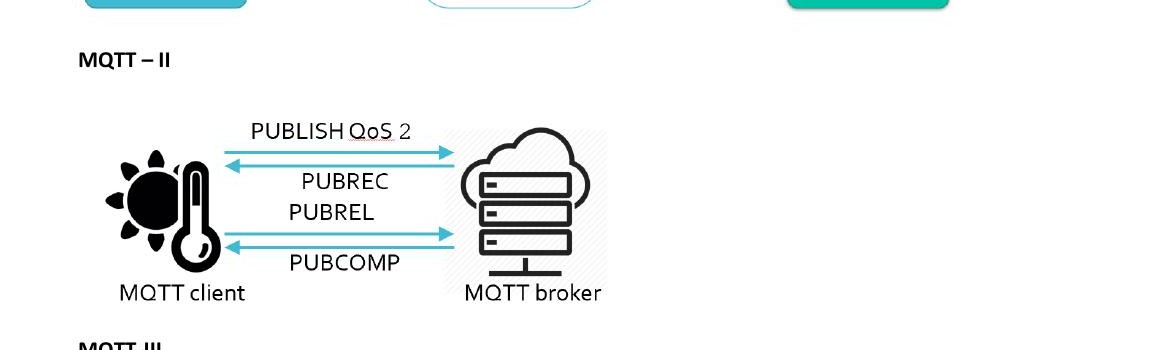
\includegraphics[keepaspectratio]{images/exam-chessa-mqtt-qos2.jpg}}
\caption{Handshake a quattro fasi del QoS 2 tra MQTT client e broker:
PUBLISH → PUBREC → PUBREL → PUBCOMP.}
\end{figure}

QoS 2 è il livello più affidabile e garantisce la consegna esattamente
una volta, senza duplicati. Il costo è un handshake a quattro fasi: 1.
\textbf{PUBLISH}: il client invia il messaggio al broker. 2.
\textbf{PUBREC} (\emph{Publish Received}): il broker conferma la
ricezione e memorizza il messaggio. 3. \textbf{PUBREL} (\emph{Publish
Release}): il client autorizza il broker a procedere con la consegna
effettiva. 4. \textbf{PUBCOMP} (\emph{Publish Complete}): il broker
conferma l'avvenuta consegna.

Il PUBREC garantisce che il messaggio non vada perso; PUBREL + PUBCOMP
garantiscono che non venga consegnato due volte. Due fasi non sarebbero
sufficienti perché si genererebbero duplicati in caso di ritrasmissione.

\newpage

\chapter{MQTT: Meccanismi di
Affidabilità}\label{mqtt-meccanismi-di-affidabilituxe0}

Questa sezione approfondisce i meccanismi che rendono il protocollo MQTT
robusto in contesti IoT: sessioni persistenti, messaggi trattenuti,
testamento e keep alive.

\section{Meccanismi di
Affidabilità}\label{meccanismi-di-affidabilituxe0}

\subsection{Sessioni Persistenti}\label{sessioni-persistenti}

Quando un dispositivo IoT si disconnette (per sleep, copertura persa,
reset), rischia di perdere le sottoscrizioni attive e i messaggi
pubblicati durante l'assenza. Le \textbf{persistent session} risolvono
questo problema.

\begin{calloutdefinition}{Sessione Persistente (Persistent Session)}

Meccanismo attivato impostando \texttt{cleanSession\ =\ false} nel
CONNECT. Il broker conserva per quel \texttt{clientId}: - Tutte le
sottoscrizioni attive - I messaggi non consegnati con QoS 1 o 2 - I
messaggi in attesa di completamento del flusso QoS 2

\end{calloutdefinition}

Alla riconnessione con lo stesso \texttt{clientId}, la sessione viene
ripristinata automaticamente. Il broker segnala la presenza di una
sessione precedente tramite il flag \emph{Session Present} nel CONNACK.

\subsection{\texorpdfstring{Messaggi Trattenuti (\emph{Retained
Messages})}{Messaggi Trattenuti (Retained Messages)}}\label{messaggi-trattenuti-retained-messages}

Nel pub/sub classico, un nuovo subscriber non sa quando arriverà il
primo messaggio. I \textbf{retained message} risolvono questo: un
messaggio pubblicato con \texttt{retainFlag\ =\ true} viene conservato
dal broker (uno per topic).

Ogni nuovo subscriber riceve immediatamente l'ultimo messaggio
trattenuto al momento dell'iscrizione, senza aspettare la prossima
pubblicazione fisiologica.

\begin{callouttip}{Esempio: stato di un dispositivo domestico}

Un dispositivo pubblica il proprio stato su
\texttt{home/devices/device1/status} con payload \texttt{"ON"} e
\texttt{retainFlag\ =\ true}. Un nuovo client che si iscrive riceve
immediatamente \texttt{"ON"}.

\end{callouttip}

\subsection{Last Will \& Testament}\label{last-will-testament}

Quando un dispositivo si disconnette \emph{normalmente} (DISCONNECT),
può notificare gli altri esplicitamente. Per le \textbf{disconnessioni
anomale} (crash, timeout, interruzione di rete) non esiste tale
possibilità.

\begin{calloutdefinition}{Last Will \& Testament}

Messaggio pre-configurato consegnato al broker al momento del CONNECT.
Se il broker rileva una disconnessione anomala, pubblica quel messaggio
automaticamente. Il testamento ha topic, payload, QoS e retained flag
propri.

\end{calloutdefinition}

Il broker invia il testamento in quattro circostanze: - Errore di I/O
sulla connessione. - Mancato invio di PINGREQ entro il keep alive. -
Chiusura brusca TCP senza DISCONNECT. - Chiusura forzata per errore di
protocollo.

Se il client si disconnette con DISCONNECT regolare, il testamento viene
scartato.

\begin{callouttip}{Pattern potente}

Un dispositivo pubblica il proprio stato (\texttt{"ON"}) come retained
message. Configura anche un testamento con payload \texttt{"OFF"} e
retain flag attivo sullo stesso topic. Se va in crash, il broker
pubblica automaticamente \texttt{"OFF"} come retained message --- tutti
i client (connessi e futuri) vedono lo stato corretto.

\end{callouttip}

\subsection{Keep Alive}\label{keep-alive}

TCP può mantenere una connessione apparentemente attiva anche quando il
peer è irraggiungibile. Il \textbf{Keep Alive} risolve questo problema:
il client dichiara un intervallo (campo a 16 bit nel CONNECT) entro cui
si impegna a inviare almeno un pacchetto.

Se non lo fa, il broker chiude la connessione e invia il testamento. Il
client invia \textbf{PINGREQ} se non ha altro traffico; il broker
risponde con \textbf{PINGRESP}. Il valore \texttt{0} disabilita il
meccanismo.

\newpage

\chapter{The ZigBee Standard --- Part 1 (Appunti
d'Esame)}\label{the-zigbee-standard-part-1-appunti-desame}

\section{Architettura a Strati e Application
Layer}\label{architettura-a-strati-e-application-layer}

\begin{figure}
\centering
\pandocbounded{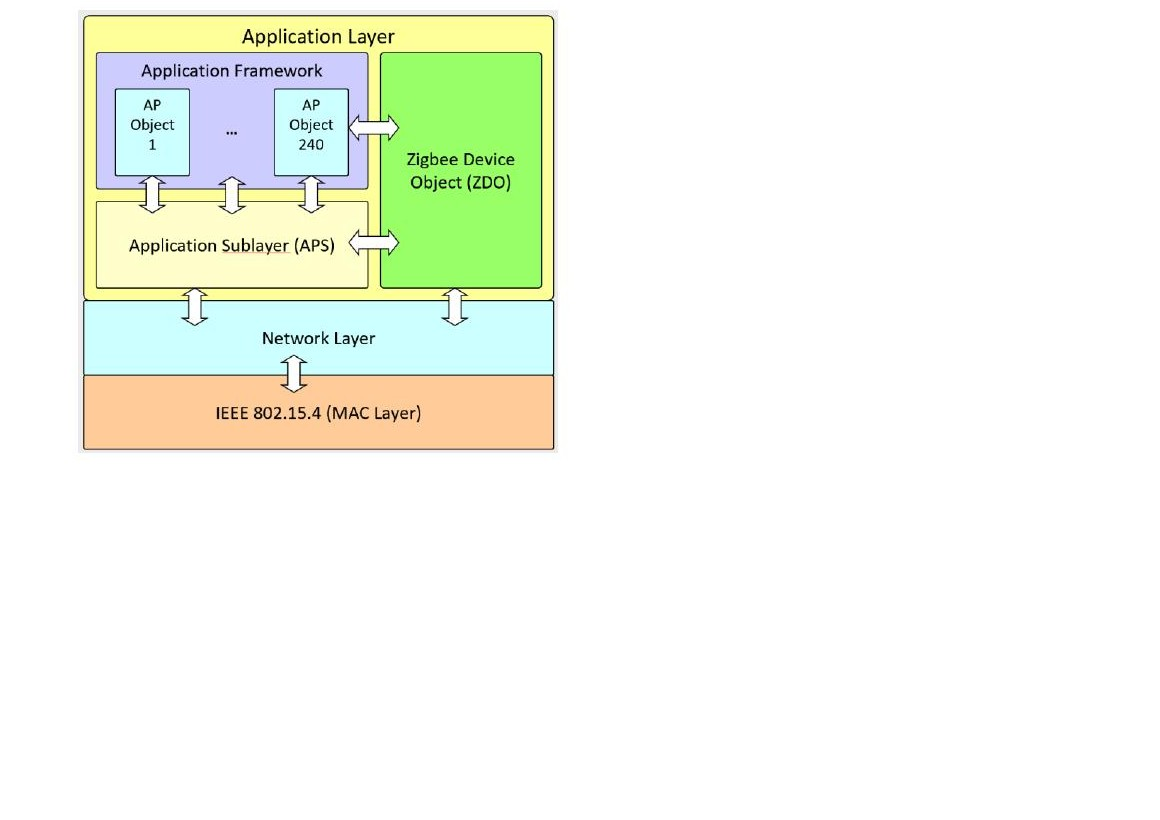
\includegraphics[keepaspectratio]{images/exam-chessa-zigbee-applayer.jpg}}
\caption{Stack protocollare ZigBee: dall'IEEE 802.15.4 (MAC) fino
all'Application Layer, con Application Framework, ZDO e APS.}
\end{figure}

ZigBee è costruito sopra lo standard IEEE 802.15.4 (PHY + MAC). Sopra
questi livelli, ZigBee aggiunge il Network Layer e l'Application Layer.
Il livello applicativo è articolato in tre componenti:

\begin{itemize}
\tightlist
\item
  \textbf{Application Framework}: ospita fino a 240 \textbf{Application
  Objects (APO)}, ciascuno associato a un endpoint (numerato da 1 a
  240). Ogni APO è identificato univocamente dalla coppia
  \texttt{\textless{}indirizzo\ di\ rete,\ endpoint\textgreater{}}. Più
  APO sullo stesso dispositivo possono corrispondere ad applicazioni
  diverse che operano simultaneamente.
\item
  \textbf{ZigBee Device Object (ZDO)}: occupa l'endpoint 0 ed è la
  componente gestionale del nodo. Fornisce:

  \begin{itemize}
  \tightlist
  \item
    Device \& Service Discovery (trova altri nodi e i loro servizi)
  \item
    Binding Management (crea/modifica le binding table dell'APS)
  \item
    Network Management (gestisce join/leave e routing table)
  \end{itemize}
\item
  \textbf{Application Support Sublayer (APS)}: fa da intermediario tra
  APO/ZDO e il Network Layer. Fornisce:

  \begin{itemize}
  \tightlist
  \item
    \emph{Data Service}: trasmissione messaggi con acknowledgment
    end-to-end
  \item
    \emph{Binding Service}: creazione di connessioni logiche tra
    endpoint
  \item
    \emph{Group Management}: indirizzamento multicast tramite Group
    Table
  \end{itemize}
\end{itemize}

L'APS filtra i pacchetti per endpoint e profile ID, scartando quelli non
destinati ad applicazioni registrate.

\begin{center}\rule{0.5\linewidth}{0.5pt}\end{center}

\section{Topologie di Rete e Routing}\label{topologie-di-rete-e-routing}

\begin{figure}
\centering
\pandocbounded{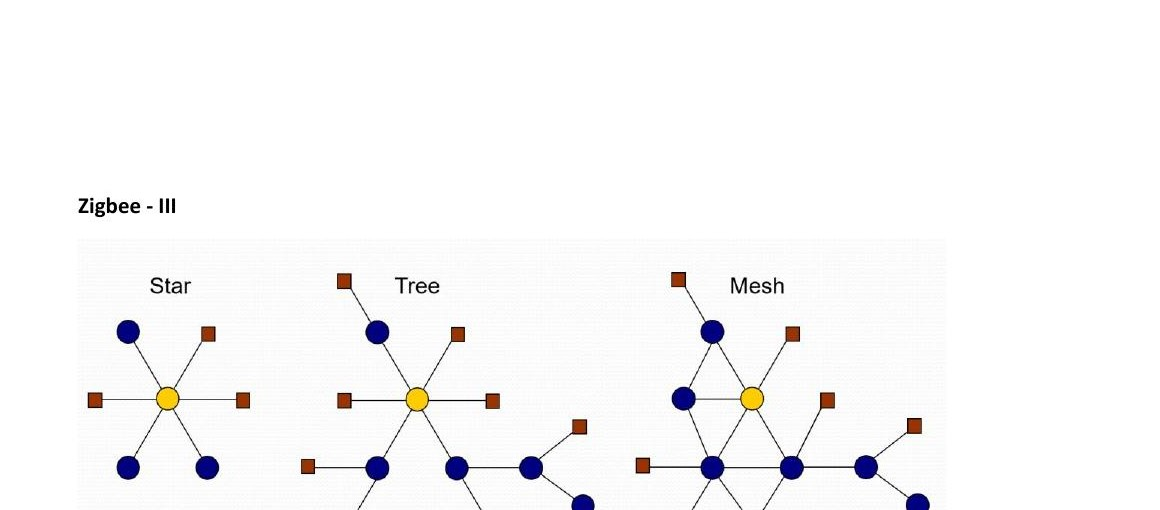
\includegraphics[keepaspectratio]{images/exam-chessa-zigbee-topologies.jpg}}
\caption{Le tre topologie ZigBee: Star (sinistra), Tree (centro), Mesh
(destra). Nodo giallo = coordinatore, nodi blu = router, nodi rossi =
end-device.}
\end{figure}

Il Network Layer definisce tre ruoli distinti: il \textbf{Network
Coordinator} (FFD che crea la rete), i \textbf{Router} (FFD con capacità
di instradamento) e gli \textbf{End-device} (RFD o FFD senza capacità di
routing).

ZigBee supporta tre topologie di rete: - \textbf{Star (Stella)}: tutti i
dispositivi comunicano direttamente con il coordinatore. Si mappa
direttamente sulla struttura IEEE 802.15.4 e supporta il meccanismo del
superframe/beacon. Semplice ma non scalabile: ogni dispositivo deve
essere nel raggio radio del coordinatore. - \textbf{Tree (Albero)}: il
coordinatore è la radice, i router sono nodi interni, gli end-device
sono foglie. Può usare il superframe. Il routing segue la struttura
gerarchica (tree routing): i pacchetti salgono verso la radice e poi
scendono verso la destinazione. Il vantaggio è la semplicità; lo
svantaggio è la rigidità e i percorsi spesso subottimali. -
\textbf{Mesh}: topologia più flessibile in cui i router possono
comunicare direttamente tra loro indipendentemente dalla struttura ad
albero. Usa mesh routing (ispirato ad AODV, Route Discovery Protocol con
RREQ/RREP). Non supporta il beaconing. È più robusto: percorsi
alternativi sono disponibili se un link cade.

\begin{callouttip}{Coesistenza}

Tree routing e Mesh routing possono coesistere nella stessa rete: ogni
router mantiene sia la logica ad albero che la routing table mesh,
passando dinamicamente dall'uno all'altro.

\end{callouttip}

\begin{center}\rule{0.5\linewidth}{0.5pt}\end{center}

\section{Ingresso in una Rete Esistente (Join through
Association)}\label{ingresso-in-una-rete-esistente-join-through-association}

\begin{figure}
\centering
\pandocbounded{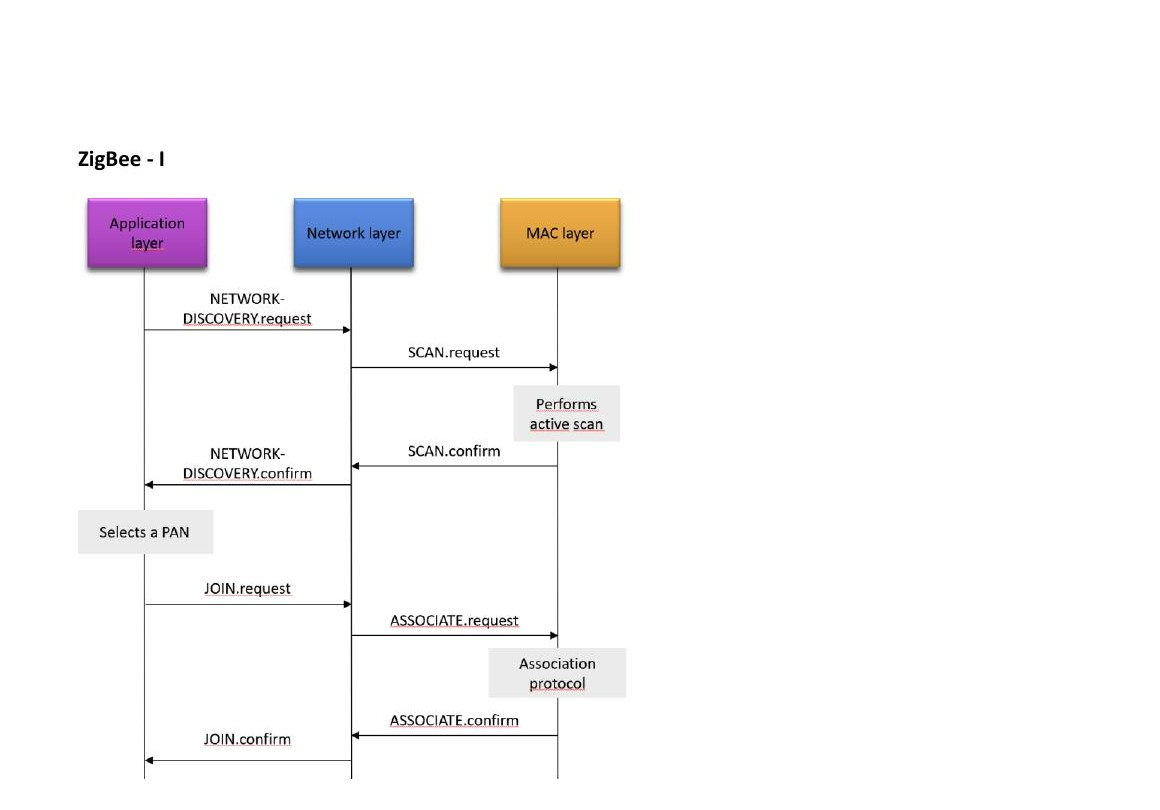
\includegraphics[keepaspectratio]{images/exam-chessa-zigbee-join.jpg}}
\caption{Sequenza di primitives tra Application Layer, Network Layer e
MAC Layer durante il processo di join di un dispositivo ZigBee.}
\end{figure}

Lo schema mostra il processo con cui un dispositivo si unisce a una rete
ZigBee esistente attraverso il meccanismo di \textbf{associazione}
(iniziativa child-side). Si tratta di un'interazione a tre livelli
(Application, Network, MAC) tramite service primitives:

\begin{enumerate}
\def\labelenumi{\arabic{enumi}.}
\tightlist
\item
  \textbf{Application layer} emette \texttt{NETWORK-DISCOVERY.request}
  al Network Layer.
\item
  \textbf{Network Layer} emette \texttt{SCAN.request} al MAC: viene
  eseguito un active scan per trovare le PAN disponibili.
\item
  \textbf{MAC} esegue lo scan e risponde con \texttt{SCAN.confirm}.
\item
  \textbf{Network Layer} risponde all'applicazione con
  \texttt{NETWORK-DISCOVERY.confirm}, che elenca le PAN trovate.
\item
  \textbf{Application layer} sceglie una PAN e invia
  \texttt{JOIN.request} al Network Layer (indicando se aggregarsi come
  router o end-device).
\item
  \textbf{Network Layer} seleziona un nodo genitore P nel vicinato
  (nelle reti a stella P è il coordinatore; in quelle ad albero/mesh P
  può essere router o coordinatore) e avvia il protocollo di
  associazione MAC tramite \texttt{ASSOCIATE.request}.
\item
  \textbf{MAC} esegue il protocollo di associazione: il
  coordinatore/router assegna un \textbf{indirizzo breve a 16 bit} al
  nuovo dispositivo.
\item
  \textbf{MAC} risponde con \texttt{ASSOCIATE.confirm} → \textbf{Network
  Layer} risponde con \texttt{JOIN.confirm} all'applicazione, rendendo
  operativo l'indirizzo per comunicazioni successive.
\end{enumerate}

\begin{center}\rule{0.5\linewidth}{0.5pt}\end{center}

\section{Struttura ad Albero e
Indirizzamento}\label{struttura-ad-albero-e-indirizzamento}

\begin{figure}
\centering
\pandocbounded{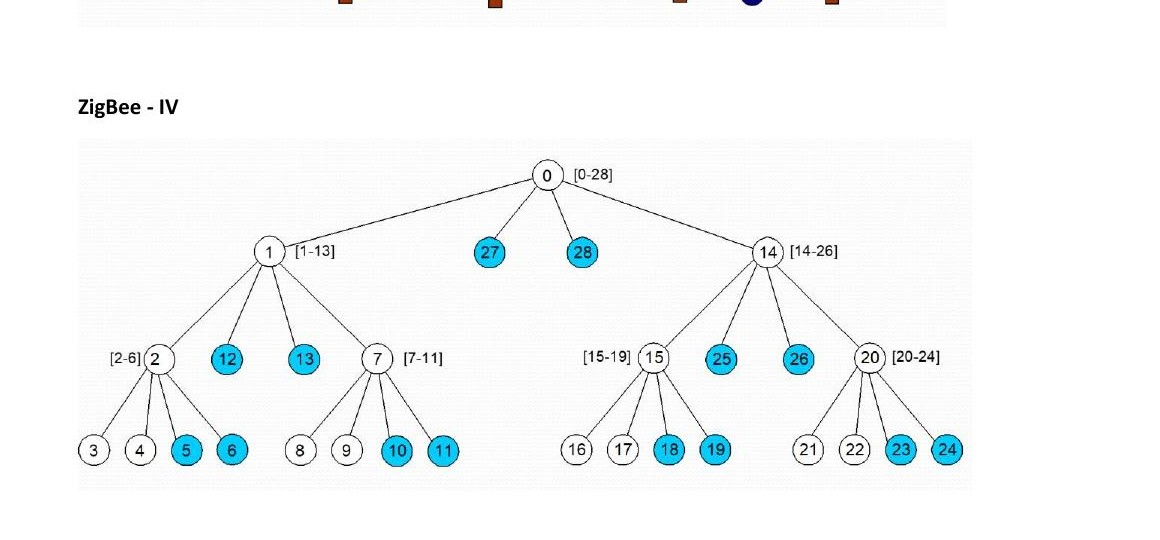
\includegraphics[keepaspectratio]{images/exam-chessa-zigbee-addrtree.jpg}}
\caption{Albero di indirizzi ZigBee con \(R_m=2\), \(D_m=2\), \(L_m=3\):
ogni nodo gestisce un intervallo di indirizzi calcolato con la formula
\(C_{skip}\).}
\end{figure}

Le relazioni genitore-figlio stabilite durante il joining costruiscono
una topologia logica ad albero, sfruttata per l'assegnazione sistematica
e decentralizzata degli indirizzi di rete. Il coordinatore viene
configurato con tre parametri: - \(R_m\): massimo numero di router figli
per nodo - \(D_m\): massimo numero di end-device figli per nodo -
\(L_m\): profondità massima dell'albero

La dimensione del blocco di indirizzi assegnato a un router a profondità
\(d\) è data dalla formula:
\[C_{skip}(d) = \begin{cases} 1 & \text{se } d = L_m \\ 1 + R_m \cdot C_{skip}(d+1) + D_m & \text{altrimenti} \end{cases}\]

Il valore \(C_{skip}(d)\) rappresenta il numero totale di indirizzi
(incluso il proprio) che ogni router alla profondità \(d\) deve
riservare per sé e per i suoi discendenti. Se un router ha indirizzo
\(A\) e si trova a profondità \(d\): - I suoi figli router ricevono in
ordine: \(A+1\), \(A+1+C_{skip}(d+1)\), \(A+1+2 \cdot C_{skip}(d+1)\),
\ldots{} - I suoi end-device ricevono gli indirizzi successivi a tutti i
blocchi riservati ai router.

\begin{callouttip}{Nell’immagine: R\_m=2, D\_m=2, L\_m=3}

- \(C_{skip}(3)=1\) - \(C_{skip}(2)=5\) - \(C_{skip}(1)=13\) -
\(C_{skip}(0)=29\) Coordinator (addr=0) gestisce {[}0--28{]}. Il primo
figlio router riceve addr=1 e gestisce {[}1--13{]}; il secondo figlio
router riceve addr=14 e gestisce {[}14--26{]}. Gli end-device del
coordinator ricevono 27 e 28.

\end{callouttip}

\textbf{Vantaggio}: Completamente decentralizzato, nessun rischio di
collisione, nessun coordinamento globale necessario.
\textbf{Svantaggio}: Rigido --- se un sottoalbero è saturo, nuovi
dispositivi non possono aggiungersi tramite quel nodo anche se ci fosse
necessità. La connettività fisica può comunque formare una mesh.

\newpage

\backmatter
\end{document}
